% Created by tikzDevice version 0.7.0 on 2014-07-23 13:33:24
% !TEX encoding = UTF-8 Unicode
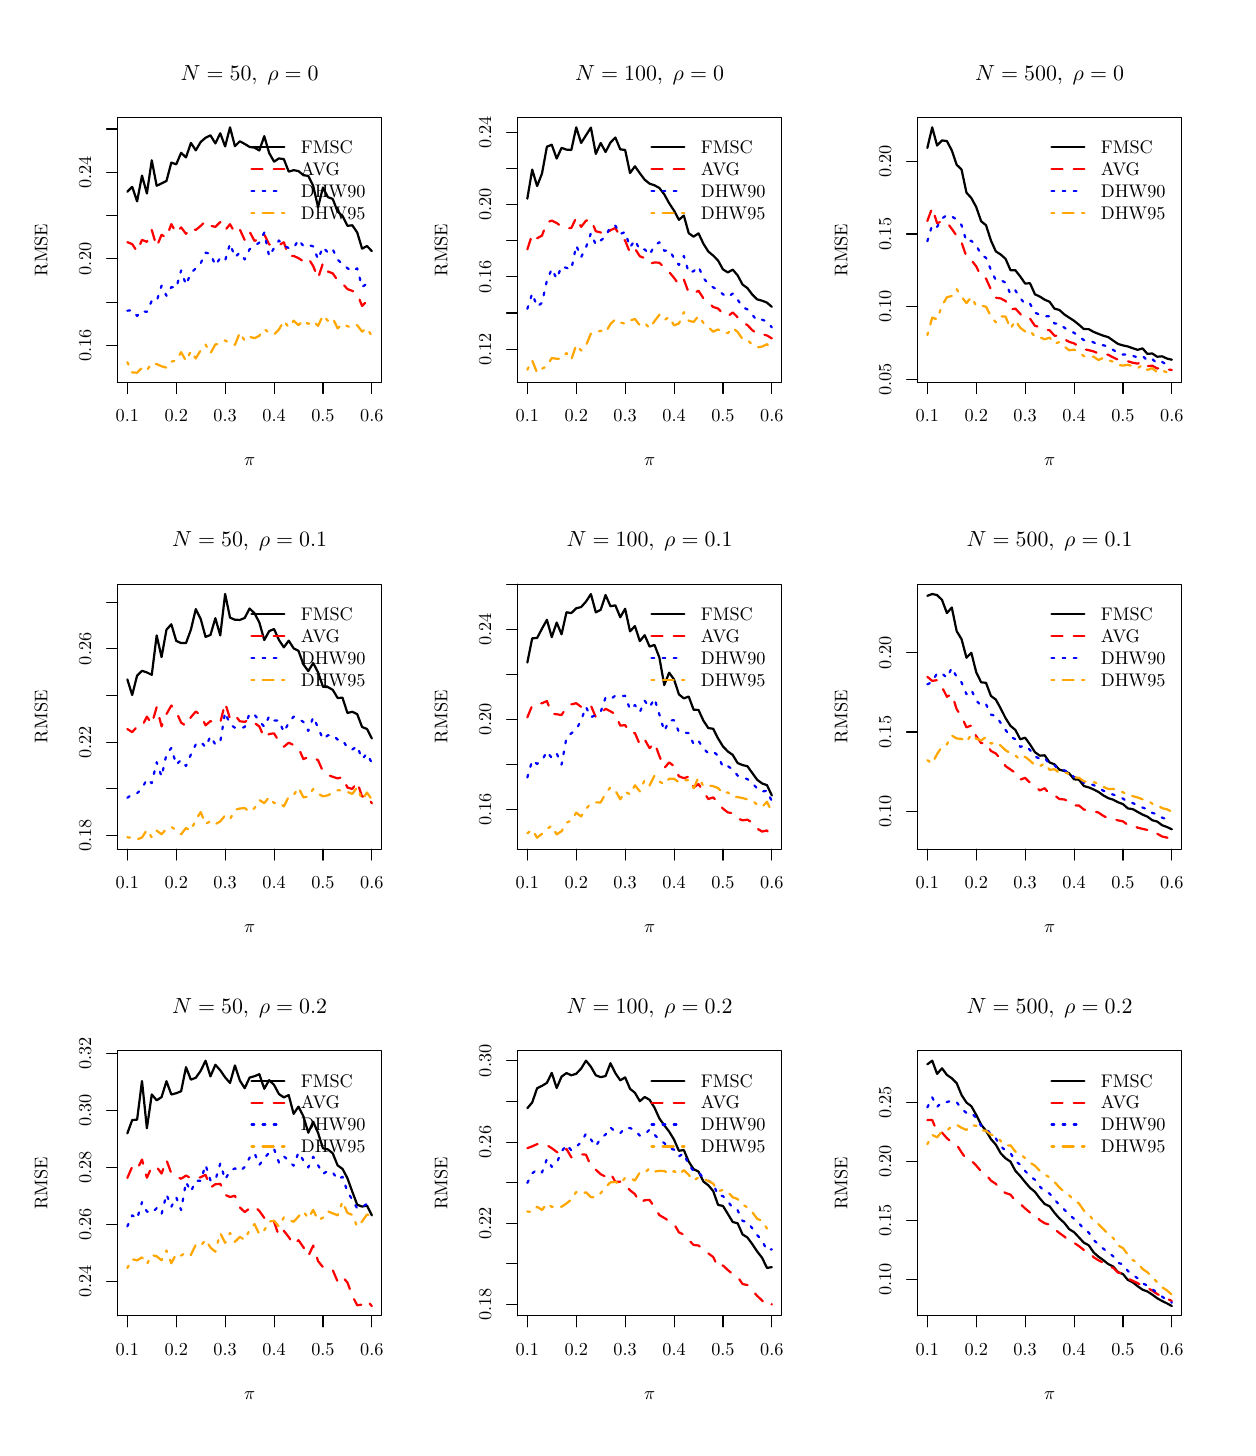
\begin{tikzpicture}[x=1pt,y=1pt]
\definecolor[named]{fillColor}{rgb}{1.00,1.00,1.00}
\path[use as bounding box,fill=fillColor,fill opacity=0.00] (0,0) rectangle (433.62,505.89);
\begin{scope}
\path[clip] ( 32.47,377.65) rectangle (127.91,473.42);
\definecolor[named]{drawColor}{rgb}{0.00,0.00,0.00}

\path[draw=drawColor,line width= 0.8pt,line join=round,line cap=round] ( 36.01,446.60) --
	( 37.77,448.37) --
	( 39.54,443.11) --
	( 41.31,452.44) --
	( 43.08,445.98) --
	( 44.84,457.95) --
	( 46.61,448.76) --
	( 48.38,449.60) --
	( 50.15,450.49) --
	( 51.91,457.13) --
	( 53.68,456.50) --
	( 55.45,460.67) --
	( 57.21,459.00) --
	( 58.98,464.24) --
	( 60.75,461.56) --
	( 62.52,464.58) --
	( 64.28,466.11) --
	( 66.05,466.99) --
	( 67.82,464.05) --
	( 69.59,467.72) --
	( 71.35,462.97) --
	( 73.12,469.87) --
	( 74.89,463.06) --
	( 76.66,464.84) --
	( 78.42,463.88) --
	( 80.19,462.79) --
	( 81.96,462.52) --
	( 83.72,461.51) --
	( 85.49,466.69) --
	( 87.26,460.60) --
	( 89.03,457.48) --
	( 90.79,458.63) --
	( 92.56,458.39) --
	( 94.33,453.87) --
	( 96.10,454.38) --
	( 97.86,454.07) --
	( 99.63,452.58) --
	(101.40,452.31) --
	(103.17,448.74) --
	(104.93,441.02) --
	(106.70,448.12) --
	(108.47,444.66) --
	(110.23,444.00) --
	(112.00,439.42) --
	(113.77,437.85) --
	(115.54,434.28) --
	(117.30,434.48) --
	(119.07,431.90) --
	(120.84,426.03) --
	(122.61,426.98) --
	(124.37,425.14);
\end{scope}
\begin{scope}
\path[clip] (  0.00,  0.00) rectangle (433.62,505.89);
\definecolor[named]{drawColor}{rgb}{0.00,0.00,0.00}

\path[draw=drawColor,line width= 0.4pt,line join=round,line cap=round] ( 36.01,377.65) -- (124.37,377.65);

\path[draw=drawColor,line width= 0.4pt,line join=round,line cap=round] ( 36.01,377.65) -- ( 36.01,373.69);

\path[draw=drawColor,line width= 0.4pt,line join=round,line cap=round] ( 53.68,377.65) -- ( 53.68,373.69);

\path[draw=drawColor,line width= 0.4pt,line join=round,line cap=round] ( 71.35,377.65) -- ( 71.35,373.69);

\path[draw=drawColor,line width= 0.4pt,line join=round,line cap=round] ( 89.03,377.65) -- ( 89.03,373.69);

\path[draw=drawColor,line width= 0.4pt,line join=round,line cap=round] (106.70,377.65) -- (106.70,373.69);

\path[draw=drawColor,line width= 0.4pt,line join=round,line cap=round] (124.37,377.65) -- (124.37,373.69);

\node[text=drawColor,anchor=base,inner sep=0pt, outer sep=0pt, scale=  0.66] at ( 36.01,363.40) {0.1};

\node[text=drawColor,anchor=base,inner sep=0pt, outer sep=0pt, scale=  0.66] at ( 53.68,363.40) {0.2};

\node[text=drawColor,anchor=base,inner sep=0pt, outer sep=0pt, scale=  0.66] at ( 71.35,363.40) {0.3};

\node[text=drawColor,anchor=base,inner sep=0pt, outer sep=0pt, scale=  0.66] at ( 89.03,363.40) {0.4};

\node[text=drawColor,anchor=base,inner sep=0pt, outer sep=0pt, scale=  0.66] at (106.70,363.40) {0.5};

\node[text=drawColor,anchor=base,inner sep=0pt, outer sep=0pt, scale=  0.66] at (124.37,363.40) {0.6};

\path[draw=drawColor,line width= 0.4pt,line join=round,line cap=round] ( 32.47,391.03) -- ( 32.47,469.27);

\path[draw=drawColor,line width= 0.4pt,line join=round,line cap=round] ( 32.47,391.03) -- ( 28.51,391.03);

\path[draw=drawColor,line width= 0.4pt,line join=round,line cap=round] ( 32.47,406.67) -- ( 28.51,406.67);

\path[draw=drawColor,line width= 0.4pt,line join=round,line cap=round] ( 32.47,422.32) -- ( 28.51,422.32);

\path[draw=drawColor,line width= 0.4pt,line join=round,line cap=round] ( 32.47,437.97) -- ( 28.51,437.97);

\path[draw=drawColor,line width= 0.4pt,line join=round,line cap=round] ( 32.47,453.62) -- ( 28.51,453.62);

\path[draw=drawColor,line width= 0.4pt,line join=round,line cap=round] ( 32.47,469.27) -- ( 28.51,469.27);

\node[text=drawColor,rotate= 90.00,anchor=base,inner sep=0pt, outer sep=0pt, scale=  0.66] at ( 22.97,391.03) {0.16};

\node[text=drawColor,rotate= 90.00,anchor=base,inner sep=0pt, outer sep=0pt, scale=  0.66] at ( 22.97,422.32) {0.20};

\node[text=drawColor,rotate= 90.00,anchor=base,inner sep=0pt, outer sep=0pt, scale=  0.66] at ( 22.97,453.62) {0.24};

\path[draw=drawColor,line width= 0.4pt,line join=round,line cap=round] ( 32.47,377.65) --
	(127.91,377.65) --
	(127.91,473.42) --
	( 32.47,473.42) --
	( 32.47,377.65);
\end{scope}
\begin{scope}
\path[clip] (  0.00,337.26) rectangle (144.54,505.89);
\definecolor[named]{drawColor}{rgb}{0.00,0.00,0.00}

\node[text=drawColor,anchor=base,inner sep=0pt, outer sep=0pt, scale=  0.79] at ( 80.19,486.92) {\bfseries $N=50, \;\rho=0$};

\node[text=drawColor,anchor=base,inner sep=0pt, outer sep=0pt, scale=  0.66] at ( 80.19,347.56) {$\pi$};

\node[text=drawColor,rotate= 90.00,anchor=base,inner sep=0pt, outer sep=0pt, scale=  0.66] at (  7.13,425.53) {RMSE};
\end{scope}
\begin{scope}
\path[clip] ( 32.47,377.65) rectangle (127.91,473.42);
\definecolor[named]{drawColor}{rgb}{1.00,0.00,0.00}

\path[draw=drawColor,line width= 0.8pt,dash pattern=on 4pt off 4pt ,line join=round,line cap=round] ( 36.01,428.38) --
	( 37.77,427.68) --
	( 39.54,425.01) --
	( 41.31,429.22) --
	( 43.08,428.49) --
	( 44.84,432.76) --
	( 46.61,426.77) --
	( 48.38,431.04) --
	( 50.15,430.04) --
	( 51.91,434.90) --
	( 53.68,431.69) --
	( 55.45,433.72) --
	( 57.21,431.37) --
	( 58.98,433.62) --
	( 60.75,432.80) --
	( 62.52,434.26) --
	( 64.28,435.98) --
	( 66.05,434.31) --
	( 67.82,433.91) --
	( 69.59,435.64) --
	( 71.35,432.68) --
	( 73.12,434.86) --
	( 74.89,431.76) --
	( 76.66,432.97) --
	( 78.42,429.14) --
	( 80.19,432.19) --
	( 81.96,428.82) --
	( 83.72,429.57) --
	( 85.49,431.21) --
	( 87.26,427.55) --
	( 89.03,427.61) --
	( 90.79,427.23) --
	( 92.56,428.35) --
	( 94.33,423.26) --
	( 96.10,423.43) --
	( 97.86,422.59) --
	( 99.63,421.46) --
	(101.40,422.58) --
	(103.17,419.74) --
	(104.93,415.37) --
	(106.70,420.80) --
	(108.47,417.77) --
	(110.23,417.11) --
	(112.00,414.57) --
	(113.77,413.42) --
	(115.54,411.42) --
	(117.30,410.78) --
	(119.07,409.71) --
	(120.84,405.32) --
	(122.61,407.17) --
	(124.37,405.38);
\definecolor[named]{drawColor}{rgb}{0.00,0.00,1.00}

\path[draw=drawColor,line width= 0.8pt,dash pattern=on 1pt off 3pt ,line join=round,line cap=round] ( 36.01,403.62) --
	( 37.77,403.79) --
	( 39.54,401.70) --
	( 41.31,403.48) --
	( 43.08,403.18) --
	( 44.84,407.21) --
	( 46.61,407.06) --
	( 48.38,412.62) --
	( 50.15,409.02) --
	( 51.91,412.16) --
	( 53.68,411.83) --
	( 55.45,418.14) --
	( 57.21,412.97) --
	( 58.98,417.27) --
	( 60.75,418.87) --
	( 62.52,420.76) --
	( 64.28,424.58) --
	( 66.05,424.20) --
	( 67.82,420.04) --
	( 69.59,422.67) --
	( 71.35,421.72) --
	( 73.12,427.85) --
	( 74.89,422.96) --
	( 76.66,424.60) --
	( 78.42,422.14) --
	( 80.19,425.82) --
	( 81.96,427.07) --
	( 83.72,428.24) --
	( 85.49,431.85) --
	( 87.26,423.24) --
	( 89.03,426.27) --
	( 90.79,428.98) --
	( 92.56,427.04) --
	( 94.33,426.28) --
	( 96.10,426.21) --
	( 97.86,429.28) --
	( 99.63,426.96) --
	(101.40,427.39) --
	(103.17,426.84) --
	(104.93,422.17) --
	(106.70,426.62) --
	(108.47,424.62) --
	(110.23,425.83) --
	(112.00,422.06) --
	(113.77,420.43) --
	(115.54,418.99) --
	(117.30,417.86) --
	(119.07,418.92) --
	(120.84,412.17) --
	(122.61,413.41) --
	(124.37,412.39);
\definecolor[named]{drawColor}{rgb}{1.00,0.65,0.00}

\path[draw=drawColor,line width= 0.8pt,dash pattern=on 1pt off 3pt on 4pt off 3pt ,line join=round,line cap=round] ( 36.01,385.02) --
	( 37.77,381.32) --
	( 39.54,381.20) --
	( 41.31,382.99) --
	( 43.08,382.07) --
	( 44.84,384.67) --
	( 46.61,384.31) --
	( 48.38,383.53) --
	( 50.15,383.03) --
	( 51.91,385.18) --
	( 53.68,385.70) --
	( 55.45,388.63) --
	( 57.21,385.49) --
	( 58.98,389.02) --
	( 60.75,386.35) --
	( 62.52,389.35) --
	( 64.28,391.36) --
	( 66.05,388.23) --
	( 67.82,391.43) --
	( 69.59,391.68) --
	( 71.35,392.90) --
	( 73.12,391.76) --
	( 74.89,391.23) --
	( 76.66,395.69) --
	( 78.42,392.78) --
	( 80.19,394.18) --
	( 81.96,393.69) --
	( 83.72,394.56) --
	( 85.49,397.03) --
	( 87.26,395.59) --
	( 89.03,394.99) --
	( 90.79,396.82) --
	( 92.56,399.94) --
	( 94.33,397.65) --
	( 96.10,400.00) --
	( 97.86,398.38) --
	( 99.63,400.10) --
	(101.40,398.84) --
	(103.17,399.86) --
	(104.93,398.13) --
	(106.70,401.89) --
	(108.47,399.97) --
	(110.23,400.95) --
	(112.00,397.23) --
	(113.77,398.87) --
	(115.54,398.00) --
	(117.30,397.54) --
	(119.07,398.40) --
	(120.84,396.03) --
	(122.61,397.35) --
	(124.37,394.40);
\definecolor[named]{drawColor}{rgb}{0.00,0.00,0.00}

\path[draw=drawColor,line width= 0.8pt,line join=round,line cap=round] ( 80.89,462.63) -- ( 92.77,462.63);
\definecolor[named]{drawColor}{rgb}{1.00,0.00,0.00}

\path[draw=drawColor,line width= 0.8pt,dash pattern=on 4pt off 4pt ,line join=round,line cap=round] ( 80.89,454.71) -- ( 92.77,454.71);
\definecolor[named]{drawColor}{rgb}{0.00,0.00,1.00}

\path[draw=drawColor,line width= 0.8pt,dash pattern=on 1pt off 3pt ,line join=round,line cap=round] ( 80.89,446.79) -- ( 92.77,446.79);
\definecolor[named]{drawColor}{rgb}{1.00,0.65,0.00}

\path[draw=drawColor,line width= 0.8pt,dash pattern=on 1pt off 3pt on 4pt off 3pt ,line join=round,line cap=round] ( 80.89,438.87) -- ( 92.77,438.87);
\definecolor[named]{drawColor}{rgb}{0.00,0.00,0.00}

\node[text=drawColor,anchor=base west,inner sep=0pt, outer sep=0pt, scale=  0.66] at ( 98.71,460.35) {FMSC};

\node[text=drawColor,anchor=base west,inner sep=0pt, outer sep=0pt, scale=  0.66] at ( 98.71,452.43) {AVG};

\node[text=drawColor,anchor=base west,inner sep=0pt, outer sep=0pt, scale=  0.66] at ( 98.71,444.51) {DHW90};

\node[text=drawColor,anchor=base west,inner sep=0pt, outer sep=0pt, scale=  0.66] at ( 98.71,436.59) {DHW95};
\end{scope}
\begin{scope}
\path[clip] (177.01,377.65) rectangle (272.45,473.42);
\definecolor[named]{drawColor}{rgb}{0.00,0.00,0.00}

\path[draw=drawColor,line width= 0.8pt,line join=round,line cap=round] (180.55,444.09) --
	(182.31,454.61) --
	(184.08,448.65) --
	(185.85,453.18) --
	(187.62,462.87) --
	(189.38,463.58) --
	(191.15,458.59) --
	(192.92,462.46) --
	(194.69,461.82) --
	(196.45,461.69) --
	(198.22,469.87) --
	(199.99,464.22) --
	(201.75,467.00) --
	(203.52,469.78) --
	(205.29,460.27) --
	(207.06,464.21) --
	(208.82,460.96) --
	(210.59,464.38) --
	(212.36,466.20) --
	(214.13,461.91) --
	(215.89,461.71) --
	(217.66,453.36) --
	(219.43,455.79) --
	(221.20,453.29) --
	(222.96,450.95) --
	(224.73,449.51) --
	(226.50,448.92) --
	(228.26,447.97) --
	(230.03,445.66) --
	(231.80,442.44) --
	(233.57,439.78) --
	(235.33,436.45) --
	(237.10,438.00) --
	(238.87,431.61) --
	(240.64,430.37) --
	(242.40,431.57) --
	(244.17,427.83) --
	(245.94,425.00) --
	(247.71,423.53) --
	(249.47,421.74) --
	(251.24,418.54) --
	(253.01,417.44) --
	(254.77,418.46) --
	(256.54,416.38) --
	(258.31,413.07) --
	(260.08,411.78) --
	(261.84,409.44) --
	(263.61,407.70) --
	(265.38,407.23) --
	(267.15,406.53) --
	(268.91,404.98);
\end{scope}
\begin{scope}
\path[clip] (  0.00,  0.00) rectangle (433.62,505.89);
\definecolor[named]{drawColor}{rgb}{0.00,0.00,0.00}

\path[draw=drawColor,line width= 0.4pt,line join=round,line cap=round] (180.55,377.65) -- (268.91,377.65);

\path[draw=drawColor,line width= 0.4pt,line join=round,line cap=round] (180.55,377.65) -- (180.55,373.69);

\path[draw=drawColor,line width= 0.4pt,line join=round,line cap=round] (198.22,377.65) -- (198.22,373.69);

\path[draw=drawColor,line width= 0.4pt,line join=round,line cap=round] (215.89,377.65) -- (215.89,373.69);

\path[draw=drawColor,line width= 0.4pt,line join=round,line cap=round] (233.57,377.65) -- (233.57,373.69);

\path[draw=drawColor,line width= 0.4pt,line join=round,line cap=round] (251.24,377.65) -- (251.24,373.69);

\path[draw=drawColor,line width= 0.4pt,line join=round,line cap=round] (268.91,377.65) -- (268.91,373.69);

\node[text=drawColor,anchor=base,inner sep=0pt, outer sep=0pt, scale=  0.66] at (180.55,363.40) {0.1};

\node[text=drawColor,anchor=base,inner sep=0pt, outer sep=0pt, scale=  0.66] at (198.22,363.40) {0.2};

\node[text=drawColor,anchor=base,inner sep=0pt, outer sep=0pt, scale=  0.66] at (215.89,363.40) {0.3};

\node[text=drawColor,anchor=base,inner sep=0pt, outer sep=0pt, scale=  0.66] at (233.57,363.40) {0.4};

\node[text=drawColor,anchor=base,inner sep=0pt, outer sep=0pt, scale=  0.66] at (251.24,363.40) {0.5};

\node[text=drawColor,anchor=base,inner sep=0pt, outer sep=0pt, scale=  0.66] at (268.91,363.40) {0.6};

\path[draw=drawColor,line width= 0.4pt,line join=round,line cap=round] (177.01,389.70) -- (177.01,468.14);

\path[draw=drawColor,line width= 0.4pt,line join=round,line cap=round] (177.01,389.70) -- (173.05,389.70);

\path[draw=drawColor,line width= 0.4pt,line join=round,line cap=round] (177.01,402.77) -- (173.05,402.77);

\path[draw=drawColor,line width= 0.4pt,line join=round,line cap=round] (177.01,415.84) -- (173.05,415.84);

\path[draw=drawColor,line width= 0.4pt,line join=round,line cap=round] (177.01,428.92) -- (173.05,428.92);

\path[draw=drawColor,line width= 0.4pt,line join=round,line cap=round] (177.01,441.99) -- (173.05,441.99);

\path[draw=drawColor,line width= 0.4pt,line join=round,line cap=round] (177.01,455.07) -- (173.05,455.07);

\path[draw=drawColor,line width= 0.4pt,line join=round,line cap=round] (177.01,468.14) -- (173.05,468.14);

\node[text=drawColor,rotate= 90.00,anchor=base,inner sep=0pt, outer sep=0pt, scale=  0.66] at (167.51,389.70) {0.12};

\node[text=drawColor,rotate= 90.00,anchor=base,inner sep=0pt, outer sep=0pt, scale=  0.66] at (167.51,415.84) {0.16};

\node[text=drawColor,rotate= 90.00,anchor=base,inner sep=0pt, outer sep=0pt, scale=  0.66] at (167.51,441.99) {0.20};

\node[text=drawColor,rotate= 90.00,anchor=base,inner sep=0pt, outer sep=0pt, scale=  0.66] at (167.51,468.14) {0.24};

\path[draw=drawColor,line width= 0.4pt,line join=round,line cap=round] (177.01,377.65) --
	(272.45,377.65) --
	(272.45,473.42) --
	(177.01,473.42) --
	(177.01,377.65);
\end{scope}
\begin{scope}
\path[clip] (144.54,337.26) rectangle (289.08,505.89);
\definecolor[named]{drawColor}{rgb}{0.00,0.00,0.00}

\node[text=drawColor,anchor=base,inner sep=0pt, outer sep=0pt, scale=  0.79] at (224.73,486.92) {\bfseries $N=100, \;\rho=0$};

\node[text=drawColor,anchor=base,inner sep=0pt, outer sep=0pt, scale=  0.66] at (224.73,347.56) {$\pi$};

\node[text=drawColor,rotate= 90.00,anchor=base,inner sep=0pt, outer sep=0pt, scale=  0.66] at (151.67,425.53) {RMSE};
\end{scope}
\begin{scope}
\path[clip] (177.01,377.65) rectangle (272.45,473.42);
\definecolor[named]{drawColor}{rgb}{1.00,0.00,0.00}

\path[draw=drawColor,line width= 0.8pt,dash pattern=on 4pt off 4pt ,line join=round,line cap=round] (180.55,425.77) --
	(182.31,431.21) --
	(184.08,429.79) --
	(185.85,430.75) --
	(187.62,435.53) --
	(189.38,436.17) --
	(191.15,435.31) --
	(192.92,434.00) --
	(194.69,433.40) --
	(196.45,433.48) --
	(198.22,437.26) --
	(199.99,433.90) --
	(201.75,436.14) --
	(203.52,436.60) --
	(205.29,432.33) --
	(207.06,431.88) --
	(208.82,430.80) --
	(210.59,432.72) --
	(212.36,433.48) --
	(214.13,430.38) --
	(215.89,428.95) --
	(217.66,424.57) --
	(219.43,426.05) --
	(221.20,423.28) --
	(222.96,422.60) --
	(224.73,420.60) --
	(226.50,421.04) --
	(228.26,420.95) --
	(230.03,419.20) --
	(231.80,417.60) --
	(233.57,415.46) --
	(235.33,413.04) --
	(237.10,414.88) --
	(238.87,410.12) --
	(240.64,409.90) --
	(242.40,410.83) --
	(244.17,408.09) --
	(245.94,406.57) --
	(247.71,404.97) --
	(249.47,404.38) --
	(251.24,402.57) --
	(253.01,401.58) --
	(254.77,403.00) --
	(256.54,401.22) --
	(258.31,399.23) --
	(260.08,398.44) --
	(261.84,396.55) --
	(263.61,395.30) --
	(265.38,395.11) --
	(267.15,394.66) --
	(268.91,393.59);
\definecolor[named]{drawColor}{rgb}{0.00,0.00,1.00}

\path[draw=drawColor,line width= 0.8pt,dash pattern=on 1pt off 3pt ,line join=round,line cap=round] (180.55,404.29) --
	(182.31,409.86) --
	(184.08,405.07) --
	(185.85,406.48) --
	(187.62,414.50) --
	(189.38,418.70) --
	(191.15,415.16) --
	(192.92,419.65) --
	(194.69,419.08) --
	(196.45,418.57) --
	(198.22,427.20) --
	(199.99,422.97) --
	(201.75,426.52) --
	(203.52,431.59) --
	(205.29,427.48) --
	(207.06,428.99) --
	(208.82,430.36) --
	(210.59,434.07) --
	(212.36,434.31) --
	(214.13,431.34) --
	(215.89,432.05) --
	(217.66,426.52) --
	(219.43,429.15) --
	(221.20,425.54) --
	(222.96,425.76) --
	(224.73,423.82) --
	(226.50,427.18) --
	(228.26,428.34) --
	(230.03,425.25) --
	(231.80,425.55) --
	(233.57,422.60) --
	(235.33,420.14) --
	(237.10,423.41) --
	(238.87,417.34) --
	(240.64,417.90) --
	(242.40,419.55) --
	(244.17,415.40) --
	(245.94,413.36) --
	(247.71,412.06) --
	(249.47,411.01) --
	(251.24,409.56) --
	(253.01,408.52) --
	(254.77,409.83) --
	(256.54,407.64) --
	(258.31,404.90) --
	(260.08,404.07) --
	(261.84,402.13) --
	(263.61,400.04) --
	(265.38,400.35) --
	(267.15,399.73) --
	(268.91,397.58);
\definecolor[named]{drawColor}{rgb}{1.00,0.65,0.00}

\path[draw=drawColor,line width= 0.8pt,dash pattern=on 1pt off 3pt on 4pt off 3pt ,line join=round,line cap=round] (180.55,382.28) --
	(182.31,385.66) --
	(184.08,381.20) --
	(185.85,382.64) --
	(187.62,383.54) --
	(189.38,386.52) --
	(191.15,386.23) --
	(192.92,386.31) --
	(194.69,388.30) --
	(196.45,385.94) --
	(198.22,391.26) --
	(199.99,389.23) --
	(201.75,391.08) --
	(203.52,395.35) --
	(205.29,395.86) --
	(207.06,396.36) --
	(208.82,395.74) --
	(210.59,398.79) --
	(212.36,400.50) --
	(214.13,399.33) --
	(215.89,398.94) --
	(217.66,400.08) --
	(219.43,400.61) --
	(221.20,398.33) --
	(222.96,399.19) --
	(224.73,397.24) --
	(226.50,399.83) --
	(228.26,402.14) --
	(230.03,400.18) --
	(231.80,401.40) --
	(233.57,398.29) --
	(235.33,399.01) --
	(237.10,403.08) --
	(238.87,399.98) --
	(240.64,399.55) --
	(242.40,401.73) --
	(244.17,399.25) --
	(245.94,397.65) --
	(247.71,396.04) --
	(249.47,396.83) --
	(251.24,395.82) --
	(253.01,395.53) --
	(254.77,397.42) --
	(256.54,395.92) --
	(258.31,393.37) --
	(260.08,393.05) --
	(261.84,391.28) --
	(263.61,390.36) --
	(265.38,390.64) --
	(267.15,391.53) --
	(268.91,389.15);
\definecolor[named]{drawColor}{rgb}{0.00,0.00,0.00}

\path[draw=drawColor,line width= 0.8pt,line join=round,line cap=round] (225.43,462.63) -- (237.31,462.63);
\definecolor[named]{drawColor}{rgb}{1.00,0.00,0.00}

\path[draw=drawColor,line width= 0.8pt,dash pattern=on 4pt off 4pt ,line join=round,line cap=round] (225.43,454.71) -- (237.31,454.71);
\definecolor[named]{drawColor}{rgb}{0.00,0.00,1.00}

\path[draw=drawColor,line width= 0.8pt,dash pattern=on 1pt off 3pt ,line join=round,line cap=round] (225.43,446.79) -- (237.31,446.79);
\definecolor[named]{drawColor}{rgb}{1.00,0.65,0.00}

\path[draw=drawColor,line width= 0.8pt,dash pattern=on 1pt off 3pt on 4pt off 3pt ,line join=round,line cap=round] (225.43,438.87) -- (237.31,438.87);
\definecolor[named]{drawColor}{rgb}{0.00,0.00,0.00}

\node[text=drawColor,anchor=base west,inner sep=0pt, outer sep=0pt, scale=  0.66] at (243.25,460.35) {FMSC};

\node[text=drawColor,anchor=base west,inner sep=0pt, outer sep=0pt, scale=  0.66] at (243.25,452.43) {AVG};

\node[text=drawColor,anchor=base west,inner sep=0pt, outer sep=0pt, scale=  0.66] at (243.25,444.51) {DHW90};

\node[text=drawColor,anchor=base west,inner sep=0pt, outer sep=0pt, scale=  0.66] at (243.25,436.59) {DHW95};
\end{scope}
\begin{scope}
\path[clip] (321.55,377.65) rectangle (416.99,473.42);
\definecolor[named]{drawColor}{rgb}{0.00,0.00,0.00}

\path[draw=drawColor,line width= 0.8pt,line join=round,line cap=round] (325.09,462.41) --
	(326.85,469.87) --
	(328.62,463.30) --
	(330.39,465.14) --
	(332.16,464.90) --
	(333.92,461.55) --
	(335.69,456.35) --
	(337.46,454.60) --
	(339.23,446.26) --
	(340.99,444.32) --
	(342.76,441.05) --
	(344.53,435.94) --
	(346.29,434.51) --
	(348.06,428.99) --
	(349.83,425.06) --
	(351.60,423.91) --
	(353.36,422.35) --
	(355.13,418.27) --
	(356.90,418.21) --
	(358.67,415.97) --
	(360.43,413.44) --
	(362.20,413.53) --
	(363.97,409.55) --
	(365.74,408.71) --
	(367.50,407.59) --
	(369.27,406.84) --
	(371.04,404.35) --
	(372.80,403.88) --
	(374.57,402.29) --
	(376.34,401.11) --
	(378.11,399.96) --
	(379.87,398.56) --
	(381.64,396.97) --
	(383.41,396.95) --
	(385.18,395.95) --
	(386.94,395.24) --
	(388.71,394.57) --
	(390.48,394.06) --
	(392.25,392.81) --
	(394.01,391.60) --
	(395.78,391.07) --
	(397.55,390.69) --
	(399.31,390.05) --
	(401.08,389.47) --
	(402.85,390.00) --
	(404.62,388.00) --
	(406.38,388.16) --
	(408.15,386.98) --
	(409.92,387.13) --
	(411.69,386.31) --
	(413.45,385.90);
\end{scope}
\begin{scope}
\path[clip] (  0.00,  0.00) rectangle (433.62,505.89);
\definecolor[named]{drawColor}{rgb}{0.00,0.00,0.00}

\path[draw=drawColor,line width= 0.4pt,line join=round,line cap=round] (325.09,377.65) -- (413.45,377.65);

\path[draw=drawColor,line width= 0.4pt,line join=round,line cap=round] (325.09,377.65) -- (325.09,373.69);

\path[draw=drawColor,line width= 0.4pt,line join=round,line cap=round] (342.76,377.65) -- (342.76,373.69);

\path[draw=drawColor,line width= 0.4pt,line join=round,line cap=round] (360.43,377.65) -- (360.43,373.69);

\path[draw=drawColor,line width= 0.4pt,line join=round,line cap=round] (378.11,377.65) -- (378.11,373.69);

\path[draw=drawColor,line width= 0.4pt,line join=round,line cap=round] (395.78,377.65) -- (395.78,373.69);

\path[draw=drawColor,line width= 0.4pt,line join=round,line cap=round] (413.45,377.65) -- (413.45,373.69);

\node[text=drawColor,anchor=base,inner sep=0pt, outer sep=0pt, scale=  0.66] at (325.09,363.40) {0.1};

\node[text=drawColor,anchor=base,inner sep=0pt, outer sep=0pt, scale=  0.66] at (342.76,363.40) {0.2};

\node[text=drawColor,anchor=base,inner sep=0pt, outer sep=0pt, scale=  0.66] at (360.43,363.40) {0.3};

\node[text=drawColor,anchor=base,inner sep=0pt, outer sep=0pt, scale=  0.66] at (378.11,363.40) {0.4};

\node[text=drawColor,anchor=base,inner sep=0pt, outer sep=0pt, scale=  0.66] at (395.78,363.40) {0.5};

\node[text=drawColor,anchor=base,inner sep=0pt, outer sep=0pt, scale=  0.66] at (413.45,363.40) {0.6};

\path[draw=drawColor,line width= 0.4pt,line join=round,line cap=round] (321.55,378.88) -- (321.55,457.55);

\path[draw=drawColor,line width= 0.4pt,line join=round,line cap=round] (321.55,378.88) -- (317.59,378.88);

\path[draw=drawColor,line width= 0.4pt,line join=round,line cap=round] (321.55,405.10) -- (317.59,405.10);

\path[draw=drawColor,line width= 0.4pt,line join=round,line cap=round] (321.55,431.33) -- (317.59,431.33);

\path[draw=drawColor,line width= 0.4pt,line join=round,line cap=round] (321.55,457.55) -- (317.59,457.55);

\node[text=drawColor,rotate= 90.00,anchor=base,inner sep=0pt, outer sep=0pt, scale=  0.66] at (312.05,378.88) {0.05};

\node[text=drawColor,rotate= 90.00,anchor=base,inner sep=0pt, outer sep=0pt, scale=  0.66] at (312.05,405.10) {0.10};

\node[text=drawColor,rotate= 90.00,anchor=base,inner sep=0pt, outer sep=0pt, scale=  0.66] at (312.05,431.33) {0.15};

\node[text=drawColor,rotate= 90.00,anchor=base,inner sep=0pt, outer sep=0pt, scale=  0.66] at (312.05,457.55) {0.20};

\path[draw=drawColor,line width= 0.4pt,line join=round,line cap=round] (321.55,377.65) --
	(416.99,377.65) --
	(416.99,473.42) --
	(321.55,473.42) --
	(321.55,377.65);
\end{scope}
\begin{scope}
\path[clip] (289.08,337.26) rectangle (433.62,505.89);
\definecolor[named]{drawColor}{rgb}{0.00,0.00,0.00}

\node[text=drawColor,anchor=base,inner sep=0pt, outer sep=0pt, scale=  0.79] at (369.27,486.92) {\bfseries $N=500, \;\rho=0$};

\node[text=drawColor,anchor=base,inner sep=0pt, outer sep=0pt, scale=  0.66] at (369.27,347.56) {$\pi$};

\node[text=drawColor,rotate= 90.00,anchor=base,inner sep=0pt, outer sep=0pt, scale=  0.66] at (296.21,425.53) {RMSE};
\end{scope}
\begin{scope}
\path[clip] (321.55,377.65) rectangle (416.99,473.42);
\definecolor[named]{drawColor}{rgb}{1.00,0.00,0.00}

\path[draw=drawColor,line width= 0.8pt,dash pattern=on 4pt off 4pt ,line join=round,line cap=round] (325.09,436.03) --
	(326.85,440.77) --
	(328.62,435.22) --
	(330.39,435.95) --
	(332.16,435.58) --
	(333.92,433.19) --
	(335.69,430.65) --
	(337.46,428.31) --
	(339.23,423.07) --
	(340.99,421.86) --
	(342.76,419.64) --
	(344.53,415.90) --
	(346.29,415.23) --
	(348.06,411.32) --
	(349.83,408.30) --
	(351.60,408.04) --
	(353.36,407.12) --
	(355.13,404.04) --
	(356.90,404.38) --
	(358.67,402.47) --
	(360.43,400.68) --
	(362.20,400.73) --
	(363.97,398.15) --
	(365.74,397.68) --
	(367.50,396.70) --
	(369.27,396.56) --
	(371.04,394.58) --
	(372.80,394.55) --
	(374.57,393.31) --
	(376.34,392.36) --
	(378.11,391.81) --
	(379.87,390.70) --
	(381.64,389.73) --
	(383.41,389.34) --
	(385.18,388.91) --
	(386.94,388.13) --
	(388.71,388.09) --
	(390.48,387.67) --
	(392.25,386.72) --
	(394.01,385.90) --
	(395.78,385.49) --
	(397.55,385.35) --
	(399.31,384.80) --
	(401.08,384.50) --
	(402.85,385.13) --
	(404.62,383.56) --
	(406.38,383.75) --
	(408.15,382.73) --
	(409.92,383.04) --
	(411.69,382.43) --
	(413.45,382.19);
\definecolor[named]{drawColor}{rgb}{0.00,0.00,1.00}

\path[draw=drawColor,line width= 0.8pt,dash pattern=on 1pt off 3pt ,line join=round,line cap=round] (325.09,428.70) --
	(326.85,434.61) --
	(328.62,433.90) --
	(330.39,436.92) --
	(332.16,438.19) --
	(333.92,437.67) --
	(335.69,436.58) --
	(337.46,434.52) --
	(339.23,428.58) --
	(340.99,428.88) --
	(342.76,427.27) --
	(344.53,423.81) --
	(346.29,422.74) --
	(348.06,418.37) --
	(349.83,414.70) --
	(351.60,414.66) --
	(353.36,413.74) --
	(355.13,409.53) --
	(356.90,410.94) --
	(358.67,408.19) --
	(360.43,405.94) --
	(362.20,406.13) --
	(363.97,402.90) --
	(365.74,402.15) --
	(367.50,401.58) --
	(369.27,401.58) --
	(371.04,398.99) --
	(372.80,398.95) --
	(374.57,397.49) --
	(376.34,396.31) --
	(378.11,395.63) --
	(379.87,394.31) --
	(381.64,392.98) --
	(383.41,392.74) --
	(385.18,392.18) --
	(386.94,391.26) --
	(388.71,391.12) --
	(390.48,390.64) --
	(392.25,389.45) --
	(394.01,388.32) --
	(395.78,387.75) --
	(397.55,387.84) --
	(399.31,387.28) --
	(401.08,386.77) --
	(402.85,387.29) --
	(404.62,385.55) --
	(406.38,386.11) --
	(408.15,384.54) --
	(409.92,385.09) --
	(411.69,384.08) --
	(413.45,383.75);
\definecolor[named]{drawColor}{rgb}{1.00,0.65,0.00}

\path[draw=drawColor,line width= 0.8pt,dash pattern=on 1pt off 3pt on 4pt off 3pt ,line join=round,line cap=round] (325.09,394.78) --
	(326.85,401.10) --
	(328.62,400.51) --
	(330.39,405.45) --
	(332.16,408.46) --
	(333.92,408.96) --
	(335.69,411.39) --
	(337.46,408.65) --
	(339.23,406.36) --
	(340.99,408.56) --
	(342.76,405.36) --
	(344.53,405.47) --
	(346.29,405.04) --
	(348.06,401.59) --
	(349.83,399.43) --
	(351.60,401.59) --
	(353.36,401.48) --
	(355.13,397.11) --
	(356.90,400.07) --
	(358.67,397.44) --
	(360.43,396.12) --
	(362.20,396.51) --
	(363.97,394.13) --
	(365.74,394.04) --
	(367.50,393.26) --
	(369.27,393.91) --
	(371.04,391.63) --
	(372.80,392.30) --
	(374.57,390.70) --
	(376.34,389.31) --
	(378.11,389.55) --
	(379.87,388.56) --
	(381.64,387.23) --
	(383.41,386.99) --
	(385.18,386.98) --
	(386.94,385.78) --
	(388.71,386.61) --
	(390.48,385.74) --
	(392.25,385.15) --
	(394.01,384.00) --
	(395.78,383.79) --
	(397.55,384.09) --
	(399.31,383.52) --
	(401.08,382.85) --
	(402.85,383.98) --
	(404.62,382.23) --
	(406.38,382.83) --
	(408.15,381.35) --
	(409.92,382.01) --
	(411.69,381.34) --
	(413.45,381.20);
\definecolor[named]{drawColor}{rgb}{0.00,0.00,0.00}

\path[draw=drawColor,line width= 0.8pt,line join=round,line cap=round] (369.97,462.63) -- (381.85,462.63);
\definecolor[named]{drawColor}{rgb}{1.00,0.00,0.00}

\path[draw=drawColor,line width= 0.8pt,dash pattern=on 4pt off 4pt ,line join=round,line cap=round] (369.97,454.71) -- (381.85,454.71);
\definecolor[named]{drawColor}{rgb}{0.00,0.00,1.00}

\path[draw=drawColor,line width= 0.8pt,dash pattern=on 1pt off 3pt ,line join=round,line cap=round] (369.97,446.79) -- (381.85,446.79);
\definecolor[named]{drawColor}{rgb}{1.00,0.65,0.00}

\path[draw=drawColor,line width= 0.8pt,dash pattern=on 1pt off 3pt on 4pt off 3pt ,line join=round,line cap=round] (369.97,438.87) -- (381.85,438.87);
\definecolor[named]{drawColor}{rgb}{0.00,0.00,0.00}

\node[text=drawColor,anchor=base west,inner sep=0pt, outer sep=0pt, scale=  0.66] at (387.79,460.35) {FMSC};

\node[text=drawColor,anchor=base west,inner sep=0pt, outer sep=0pt, scale=  0.66] at (387.79,452.43) {AVG};

\node[text=drawColor,anchor=base west,inner sep=0pt, outer sep=0pt, scale=  0.66] at (387.79,444.51) {DHW90};

\node[text=drawColor,anchor=base west,inner sep=0pt, outer sep=0pt, scale=  0.66] at (387.79,436.59) {DHW95};
\end{scope}
\begin{scope}
\path[clip] ( 32.47,209.02) rectangle (127.91,304.79);
\definecolor[named]{drawColor}{rgb}{0.00,0.00,0.00}

\path[draw=drawColor,line width= 0.8pt,line join=round,line cap=round] ( 36.01,270.39) --
	( 37.77,264.75) --
	( 39.54,271.76) --
	( 41.31,273.48) --
	( 43.08,272.90) --
	( 44.84,272.02) --
	( 46.61,286.28) --
	( 48.38,278.44) --
	( 50.15,288.33) --
	( 51.91,290.32) --
	( 53.68,284.30) --
	( 55.45,283.50) --
	( 57.21,283.50) --
	( 58.98,288.36) --
	( 60.75,295.77) --
	( 62.52,292.21) --
	( 64.28,285.75) --
	( 66.05,286.44) --
	( 67.82,292.50) --
	( 69.59,286.28) --
	( 71.35,301.24) --
	( 73.12,292.72) --
	( 74.89,291.93) --
	( 76.66,291.88) --
	( 78.42,292.58) --
	( 80.19,295.99) --
	( 81.96,294.30) --
	( 83.72,290.93) --
	( 85.49,284.60) --
	( 87.26,287.83) --
	( 89.03,288.59) --
	( 90.79,284.65) --
	( 92.56,281.97) --
	( 94.33,284.40) --
	( 96.10,281.61) --
	( 97.86,280.71) --
	( 99.63,275.80) --
	(101.40,273.40) --
	(103.17,276.30) --
	(104.93,272.94) --
	(106.70,267.73) --
	(108.47,267.61) --
	(110.23,266.63) --
	(112.00,263.68) --
	(113.77,263.75) --
	(115.54,258.26) --
	(117.30,258.68) --
	(119.07,257.85) --
	(120.84,253.19) --
	(122.61,252.47) --
	(124.37,249.04);
\end{scope}
\begin{scope}
\path[clip] (  0.00,  0.00) rectangle (433.62,505.89);
\definecolor[named]{drawColor}{rgb}{0.00,0.00,0.00}

\path[draw=drawColor,line width= 0.4pt,line join=round,line cap=round] ( 36.01,209.02) -- (124.37,209.02);

\path[draw=drawColor,line width= 0.4pt,line join=round,line cap=round] ( 36.01,209.02) -- ( 36.01,205.06);

\path[draw=drawColor,line width= 0.4pt,line join=round,line cap=round] ( 53.68,209.02) -- ( 53.68,205.06);

\path[draw=drawColor,line width= 0.4pt,line join=round,line cap=round] ( 71.35,209.02) -- ( 71.35,205.06);

\path[draw=drawColor,line width= 0.4pt,line join=round,line cap=round] ( 89.03,209.02) -- ( 89.03,205.06);

\path[draw=drawColor,line width= 0.4pt,line join=round,line cap=round] (106.70,209.02) -- (106.70,205.06);

\path[draw=drawColor,line width= 0.4pt,line join=round,line cap=round] (124.37,209.02) -- (124.37,205.06);

\node[text=drawColor,anchor=base,inner sep=0pt, outer sep=0pt, scale=  0.66] at ( 36.01,194.77) {0.1};

\node[text=drawColor,anchor=base,inner sep=0pt, outer sep=0pt, scale=  0.66] at ( 53.68,194.77) {0.2};

\node[text=drawColor,anchor=base,inner sep=0pt, outer sep=0pt, scale=  0.66] at ( 71.35,194.77) {0.3};

\node[text=drawColor,anchor=base,inner sep=0pt, outer sep=0pt, scale=  0.66] at ( 89.03,194.77) {0.4};

\node[text=drawColor,anchor=base,inner sep=0pt, outer sep=0pt, scale=  0.66] at (106.70,194.77) {0.5};

\node[text=drawColor,anchor=base,inner sep=0pt, outer sep=0pt, scale=  0.66] at (124.37,194.77) {0.6};

\path[draw=drawColor,line width= 0.4pt,line join=round,line cap=round] ( 32.47,213.96) -- ( 32.47,298.28);

\path[draw=drawColor,line width= 0.4pt,line join=round,line cap=round] ( 32.47,213.96) -- ( 28.51,213.96);

\path[draw=drawColor,line width= 0.4pt,line join=round,line cap=round] ( 32.47,230.83) -- ( 28.51,230.83);

\path[draw=drawColor,line width= 0.4pt,line join=round,line cap=round] ( 32.47,247.69) -- ( 28.51,247.69);

\path[draw=drawColor,line width= 0.4pt,line join=round,line cap=round] ( 32.47,264.55) -- ( 28.51,264.55);

\path[draw=drawColor,line width= 0.4pt,line join=round,line cap=round] ( 32.47,281.42) -- ( 28.51,281.42);

\path[draw=drawColor,line width= 0.4pt,line join=round,line cap=round] ( 32.47,298.28) -- ( 28.51,298.28);

\node[text=drawColor,rotate= 90.00,anchor=base,inner sep=0pt, outer sep=0pt, scale=  0.66] at ( 22.97,213.96) {0.18};

\node[text=drawColor,rotate= 90.00,anchor=base,inner sep=0pt, outer sep=0pt, scale=  0.66] at ( 22.97,247.69) {0.22};

\node[text=drawColor,rotate= 90.00,anchor=base,inner sep=0pt, outer sep=0pt, scale=  0.66] at ( 22.97,281.42) {0.26};

\path[draw=drawColor,line width= 0.4pt,line join=round,line cap=round] ( 32.47,209.02) --
	(127.91,209.02) --
	(127.91,304.79) --
	( 32.47,304.79) --
	( 32.47,209.02);
\end{scope}
\begin{scope}
\path[clip] (  0.00,168.63) rectangle (144.54,337.26);
\definecolor[named]{drawColor}{rgb}{0.00,0.00,0.00}

\node[text=drawColor,anchor=base,inner sep=0pt, outer sep=0pt, scale=  0.79] at ( 80.19,318.29) {\bfseries $N=50, \;\rho=0.1$};

\node[text=drawColor,anchor=base,inner sep=0pt, outer sep=0pt, scale=  0.66] at ( 80.19,178.93) {$\pi$};

\node[text=drawColor,rotate= 90.00,anchor=base,inner sep=0pt, outer sep=0pt, scale=  0.66] at (  7.13,256.90) {RMSE};
\end{scope}
\begin{scope}
\path[clip] ( 32.47,209.02) rectangle (127.91,304.79);
\definecolor[named]{drawColor}{rgb}{1.00,0.00,0.00}

\path[draw=drawColor,line width= 0.8pt,dash pattern=on 4pt off 4pt ,line join=round,line cap=round] ( 36.01,252.46) --
	( 37.77,251.32) --
	( 39.54,253.31) --
	( 41.31,253.38) --
	( 43.08,256.94) --
	( 44.84,254.28) --
	( 46.61,260.34) --
	( 48.38,253.41) --
	( 50.15,257.85) --
	( 51.91,260.94) --
	( 53.68,258.71) --
	( 55.45,254.77) --
	( 57.21,253.61) --
	( 58.98,256.74) --
	( 60.75,258.77) --
	( 62.52,257.53) --
	( 64.28,253.79) --
	( 66.05,255.31) --
	( 67.82,254.79) --
	( 69.59,254.77) --
	( 71.35,261.86) --
	( 73.12,256.23) --
	( 74.89,257.49) --
	( 76.66,255.26) --
	( 78.42,255.04) --
	( 80.19,255.95) --
	( 81.96,254.66) --
	( 83.72,253.37) --
	( 85.49,249.31) --
	( 87.26,250.65) --
	( 89.03,250.89) --
	( 90.79,247.95) --
	( 92.56,246.05) --
	( 94.33,247.51) --
	( 96.10,246.67) --
	( 97.86,245.65) --
	( 99.63,241.57) --
	(101.40,242.38) --
	(103.17,242.19) --
	(104.93,241.17) --
	(106.70,237.10) --
	(108.47,235.86) --
	(110.23,235.19) --
	(112.00,234.60) --
	(113.77,235.11) --
	(115.54,231.30) --
	(117.30,230.81) --
	(119.07,233.34) --
	(120.84,228.03) --
	(122.61,228.48) --
	(124.37,225.58);
\definecolor[named]{drawColor}{rgb}{0.00,0.00,1.00}

\path[draw=drawColor,line width= 0.8pt,dash pattern=on 1pt off 3pt ,line join=round,line cap=round] ( 36.01,227.59) --
	( 37.77,228.86) --
	( 39.54,229.25) --
	( 41.31,230.91) --
	( 43.08,234.37) --
	( 44.84,232.90) --
	( 46.61,240.46) --
	( 48.38,235.30) --
	( 50.15,243.31) --
	( 51.91,245.60) --
	( 53.68,239.60) --
	( 55.45,241.31) --
	( 57.21,239.08) --
	( 58.98,243.24) --
	( 60.75,246.90) --
	( 62.52,247.83) --
	( 64.28,245.95) --
	( 66.05,249.84) --
	( 67.82,246.85) --
	( 69.59,247.82) --
	( 71.35,258.46) --
	( 73.12,254.12) --
	( 74.89,252.93) --
	( 76.66,252.59) --
	( 78.42,253.18) --
	( 80.19,258.07) --
	( 81.96,257.65) --
	( 83.72,255.37) --
	( 85.49,253.27) --
	( 87.26,257.07) --
	( 89.03,255.49) --
	( 90.79,255.54) --
	( 92.56,251.36) --
	( 94.33,254.70) --
	( 96.10,256.94) --
	( 97.86,256.12) --
	( 99.63,255.02) --
	(101.40,251.78) --
	(103.17,256.74) --
	(104.93,252.98) --
	(106.70,248.82) --
	(108.47,250.17) --
	(110.23,250.35) --
	(112.00,248.63) --
	(113.77,248.57) --
	(115.54,245.61) --
	(117.30,245.04) --
	(119.07,246.30) --
	(120.84,241.59) --
	(122.61,243.59) --
	(124.37,240.14);
\definecolor[named]{drawColor}{rgb}{1.00,0.65,0.00}

\path[draw=drawColor,line width= 0.8pt,dash pattern=on 1pt off 3pt on 4pt off 3pt ,line join=round,line cap=round] ( 36.01,213.35) --
	( 37.77,213.10) --
	( 39.54,212.57) --
	( 41.31,213.24) --
	( 43.08,216.01) --
	( 44.84,213.30) --
	( 46.61,215.75) --
	( 48.38,214.42) --
	( 50.15,216.42) --
	( 51.91,217.07) --
	( 53.68,215.94) --
	( 55.45,214.42) --
	( 57.21,216.69) --
	( 58.98,215.72) --
	( 60.75,219.67) --
	( 62.52,222.44) --
	( 64.28,218.11) --
	( 66.05,219.19) --
	( 67.82,218.08) --
	( 69.59,219.07) --
	( 71.35,221.23) --
	( 73.12,219.90) --
	( 74.89,223.22) --
	( 76.66,223.73) --
	( 78.42,223.90) --
	( 80.19,222.51) --
	( 81.96,223.86) --
	( 83.72,226.79) --
	( 85.49,225.68) --
	( 87.26,227.87) --
	( 89.03,225.69) --
	( 90.79,226.00) --
	( 92.56,224.48) --
	( 94.33,228.05) --
	( 96.10,228.51) --
	( 97.86,231.30) --
	( 99.63,227.74) --
	(101.40,228.05) --
	(103.17,230.78) --
	(104.93,229.17) --
	(106.70,228.11) --
	(108.47,228.50) --
	(110.23,229.39) --
	(112.00,230.29) --
	(113.77,230.32) --
	(115.54,229.73) --
	(117.30,228.99) --
	(119.07,231.39) --
	(120.84,226.85) --
	(122.61,229.51) --
	(124.37,226.93);
\definecolor[named]{drawColor}{rgb}{0.00,0.00,0.00}

\path[draw=drawColor,line width= 0.8pt,line join=round,line cap=round] ( 80.89,294.00) -- ( 92.77,294.00);
\definecolor[named]{drawColor}{rgb}{1.00,0.00,0.00}

\path[draw=drawColor,line width= 0.8pt,dash pattern=on 4pt off 4pt ,line join=round,line cap=round] ( 80.89,286.08) -- ( 92.77,286.08);
\definecolor[named]{drawColor}{rgb}{0.00,0.00,1.00}

\path[draw=drawColor,line width= 0.8pt,dash pattern=on 1pt off 3pt ,line join=round,line cap=round] ( 80.89,278.16) -- ( 92.77,278.16);
\definecolor[named]{drawColor}{rgb}{1.00,0.65,0.00}

\path[draw=drawColor,line width= 0.8pt,dash pattern=on 1pt off 3pt on 4pt off 3pt ,line join=round,line cap=round] ( 80.89,270.24) -- ( 92.77,270.24);
\definecolor[named]{drawColor}{rgb}{0.00,0.00,0.00}

\node[text=drawColor,anchor=base west,inner sep=0pt, outer sep=0pt, scale=  0.66] at ( 98.71,291.72) {FMSC};

\node[text=drawColor,anchor=base west,inner sep=0pt, outer sep=0pt, scale=  0.66] at ( 98.71,283.80) {AVG};

\node[text=drawColor,anchor=base west,inner sep=0pt, outer sep=0pt, scale=  0.66] at ( 98.71,275.88) {DHW90};

\node[text=drawColor,anchor=base west,inner sep=0pt, outer sep=0pt, scale=  0.66] at ( 98.71,267.96) {DHW95};
\end{scope}
\begin{scope}
\path[clip] (177.01,209.02) rectangle (272.45,304.79);
\definecolor[named]{drawColor}{rgb}{0.00,0.00,0.00}

\path[draw=drawColor,line width= 0.8pt,line join=round,line cap=round] (180.55,276.49) --
	(182.31,285.23) --
	(184.08,285.36) --
	(185.85,288.72) --
	(187.62,291.92) --
	(189.38,285.67) --
	(191.15,290.93) --
	(192.92,286.68) --
	(194.69,294.64) --
	(196.45,294.35) --
	(198.22,296.08) --
	(199.99,296.53) --
	(201.75,298.49) --
	(203.52,301.24) --
	(205.29,294.64) --
	(207.06,295.53) --
	(208.82,300.88) --
	(210.59,296.82) --
	(212.36,297.13) --
	(214.13,292.84) --
	(215.89,295.91) --
	(217.66,287.74) --
	(219.43,289.66) --
	(221.20,284.22) --
	(222.96,286.35) --
	(224.73,282.24) --
	(226.50,282.85) --
	(228.26,278.29) --
	(230.03,268.34) --
	(231.80,272.82) --
	(233.57,270.36) --
	(235.33,264.97) --
	(237.10,263.53) --
	(238.87,264.19) --
	(240.64,259.41) --
	(242.40,259.36) --
	(244.17,255.48) --
	(245.94,252.79) --
	(247.71,252.54) --
	(249.47,249.06) --
	(251.24,246.17) --
	(253.01,244.34) --
	(254.77,243.10) --
	(256.54,240.15) --
	(258.31,239.43) --
	(260.08,239.00) --
	(261.84,236.56) --
	(263.61,234.11) --
	(265.38,232.79) --
	(267.15,232.17) --
	(268.91,228.43);
\end{scope}
\begin{scope}
\path[clip] (  0.00,  0.00) rectangle (433.62,505.89);
\definecolor[named]{drawColor}{rgb}{0.00,0.00,0.00}

\path[draw=drawColor,line width= 0.4pt,line join=round,line cap=round] (180.55,209.02) -- (268.91,209.02);

\path[draw=drawColor,line width= 0.4pt,line join=round,line cap=round] (180.55,209.02) -- (180.55,205.06);

\path[draw=drawColor,line width= 0.4pt,line join=round,line cap=round] (198.22,209.02) -- (198.22,205.06);

\path[draw=drawColor,line width= 0.4pt,line join=round,line cap=round] (215.89,209.02) -- (215.89,205.06);

\path[draw=drawColor,line width= 0.4pt,line join=round,line cap=round] (233.57,209.02) -- (233.57,205.06);

\path[draw=drawColor,line width= 0.4pt,line join=round,line cap=round] (251.24,209.02) -- (251.24,205.06);

\path[draw=drawColor,line width= 0.4pt,line join=round,line cap=round] (268.91,209.02) -- (268.91,205.06);

\node[text=drawColor,anchor=base,inner sep=0pt, outer sep=0pt, scale=  0.66] at (180.55,194.77) {0.1};

\node[text=drawColor,anchor=base,inner sep=0pt, outer sep=0pt, scale=  0.66] at (198.22,194.77) {0.2};

\node[text=drawColor,anchor=base,inner sep=0pt, outer sep=0pt, scale=  0.66] at (215.89,194.77) {0.3};

\node[text=drawColor,anchor=base,inner sep=0pt, outer sep=0pt, scale=  0.66] at (233.57,194.77) {0.4};

\node[text=drawColor,anchor=base,inner sep=0pt, outer sep=0pt, scale=  0.66] at (251.24,194.77) {0.5};

\node[text=drawColor,anchor=base,inner sep=0pt, outer sep=0pt, scale=  0.66] at (268.91,194.77) {0.6};

\path[draw=drawColor,line width= 0.4pt,line join=round,line cap=round] (177.01,223.46) -- (177.01,304.77);

\path[draw=drawColor,line width= 0.4pt,line join=round,line cap=round] (177.01,223.46) -- (173.05,223.46);

\path[draw=drawColor,line width= 0.4pt,line join=round,line cap=round] (177.01,239.72) -- (173.05,239.72);

\path[draw=drawColor,line width= 0.4pt,line join=round,line cap=round] (177.01,255.98) -- (173.05,255.98);

\path[draw=drawColor,line width= 0.4pt,line join=round,line cap=round] (177.01,272.24) -- (173.05,272.24);

\path[draw=drawColor,line width= 0.4pt,line join=round,line cap=round] (177.01,288.51) -- (173.05,288.51);

\path[draw=drawColor,line width= 0.4pt,line join=round,line cap=round] (177.01,304.77) -- (173.05,304.77);

\node[text=drawColor,rotate= 90.00,anchor=base,inner sep=0pt, outer sep=0pt, scale=  0.66] at (167.51,223.46) {0.16};

\node[text=drawColor,rotate= 90.00,anchor=base,inner sep=0pt, outer sep=0pt, scale=  0.66] at (167.51,255.98) {0.20};

\node[text=drawColor,rotate= 90.00,anchor=base,inner sep=0pt, outer sep=0pt, scale=  0.66] at (167.51,288.51) {0.24};

\path[draw=drawColor,line width= 0.4pt,line join=round,line cap=round] (177.01,209.02) --
	(272.45,209.02) --
	(272.45,304.79) --
	(177.01,304.79) --
	(177.01,209.02);
\end{scope}
\begin{scope}
\path[clip] (144.54,168.63) rectangle (289.08,337.26);
\definecolor[named]{drawColor}{rgb}{0.00,0.00,0.00}

\node[text=drawColor,anchor=base,inner sep=0pt, outer sep=0pt, scale=  0.79] at (224.73,318.29) {\bfseries $N=100, \;\rho=0.1$};

\node[text=drawColor,anchor=base,inner sep=0pt, outer sep=0pt, scale=  0.66] at (224.73,178.93) {$\pi$};

\node[text=drawColor,rotate= 90.00,anchor=base,inner sep=0pt, outer sep=0pt, scale=  0.66] at (151.67,256.90) {RMSE};
\end{scope}
\begin{scope}
\path[clip] (177.01,209.02) rectangle (272.45,304.79);
\definecolor[named]{drawColor}{rgb}{1.00,0.00,0.00}

\path[draw=drawColor,line width= 0.8pt,dash pattern=on 4pt off 4pt ,line join=round,line cap=round] (180.55,256.65) --
	(182.31,260.98) --
	(184.08,261.50) --
	(185.85,261.77) --
	(187.62,262.55) --
	(189.38,258.01) --
	(191.15,257.78) --
	(192.92,257.52) --
	(194.69,260.24) --
	(196.45,261.35) --
	(198.22,261.79) --
	(199.99,260.45) --
	(201.75,260.87) --
	(203.52,260.92) --
	(205.29,256.73) --
	(207.06,258.02) --
	(208.82,259.78) --
	(210.59,258.85) --
	(212.36,257.81) --
	(214.13,253.68) --
	(215.89,253.87) --
	(217.66,250.94) --
	(219.43,251.05) --
	(221.20,246.78) --
	(222.96,248.63) --
	(224.73,245.54) --
	(226.50,247.50) --
	(228.26,242.70) --
	(230.03,238.32) --
	(231.80,240.40) --
	(233.57,239.04) --
	(235.33,235.38) --
	(237.10,234.70) --
	(238.87,235.22) --
	(240.64,231.32) --
	(242.40,232.56) --
	(244.17,229.89) --
	(245.94,227.14) --
	(247.71,227.76) --
	(249.47,225.88) --
	(251.24,223.68) --
	(253.01,222.31) --
	(254.77,222.03) --
	(256.54,220.14) --
	(258.31,219.47) --
	(260.08,219.68) --
	(261.84,218.59) --
	(263.61,216.46) --
	(265.38,215.39) --
	(267.15,215.81) --
	(268.91,212.57);
\definecolor[named]{drawColor}{rgb}{0.00,0.00,1.00}

\path[draw=drawColor,line width= 0.8pt,dash pattern=on 1pt off 3pt ,line join=round,line cap=round] (180.55,234.95) --
	(182.31,241.12) --
	(184.08,239.85) --
	(185.85,241.13) --
	(187.62,244.32) --
	(189.38,242.01) --
	(191.15,243.66) --
	(192.92,239.60) --
	(194.69,249.35) --
	(196.45,250.93) --
	(198.22,252.22) --
	(199.99,255.68) --
	(201.75,260.41) --
	(203.52,256.72) --
	(205.29,257.51) --
	(207.06,258.64) --
	(208.82,263.83) --
	(210.59,263.22) --
	(212.36,264.52) --
	(214.13,264.34) --
	(215.89,264.46) --
	(217.66,259.52) --
	(219.43,261.11) --
	(221.20,258.55) --
	(222.96,262.65) --
	(224.73,260.30) --
	(226.50,263.46) --
	(228.26,257.72) --
	(230.03,251.69) --
	(231.80,255.55) --
	(233.57,255.61) --
	(235.33,251.35) --
	(237.10,251.13) --
	(238.87,250.99) --
	(240.64,246.95) --
	(242.40,248.24) --
	(244.17,245.32) --
	(245.94,243.76) --
	(247.71,244.27) --
	(249.47,242.86) --
	(251.24,238.66) --
	(253.01,239.02) --
	(254.77,237.88) --
	(256.54,235.62) --
	(258.31,234.93) --
	(260.08,234.36) --
	(261.84,232.81) --
	(263.61,230.99) --
	(265.38,229.85) --
	(267.15,230.18) --
	(268.91,226.30);
\definecolor[named]{drawColor}{rgb}{1.00,0.65,0.00}

\path[draw=drawColor,line width= 0.8pt,dash pattern=on 1pt off 3pt on 4pt off 3pt ,line join=round,line cap=round] (180.55,214.77) --
	(182.31,216.11) --
	(184.08,213.17) --
	(185.85,214.60) --
	(187.62,216.37) --
	(189.38,217.50) --
	(191.15,214.37) --
	(192.92,215.53) --
	(194.69,218.55) --
	(196.45,219.45) --
	(198.22,222.21) --
	(199.99,220.87) --
	(201.75,223.62) --
	(203.52,225.52) --
	(205.29,225.96) --
	(207.06,225.92) --
	(208.82,229.18) --
	(210.59,231.41) --
	(212.36,230.22) --
	(214.13,227.06) --
	(215.89,229.87) --
	(217.66,228.82) --
	(219.43,232.14) --
	(221.20,229.92) --
	(222.96,234.06) --
	(224.73,232.07) --
	(226.50,235.61) --
	(228.26,233.51) --
	(230.03,232.46) --
	(231.80,234.51) --
	(233.57,234.47) --
	(235.33,233.17) --
	(237.10,233.91) --
	(238.87,233.99) --
	(240.64,231.09) --
	(242.40,234.97) --
	(244.17,231.83) --
	(245.94,232.07) --
	(247.71,231.79) --
	(249.47,231.14) --
	(251.24,229.11) --
	(253.01,229.56) --
	(254.77,227.93) --
	(256.54,227.85) --
	(258.31,227.52) --
	(260.08,227.02) --
	(261.84,226.49) --
	(263.61,225.18) --
	(265.38,224.30) --
	(267.15,226.18) --
	(268.91,222.44);
\definecolor[named]{drawColor}{rgb}{0.00,0.00,0.00}

\path[draw=drawColor,line width= 0.8pt,line join=round,line cap=round] (225.43,294.00) -- (237.31,294.00);
\definecolor[named]{drawColor}{rgb}{1.00,0.00,0.00}

\path[draw=drawColor,line width= 0.8pt,dash pattern=on 4pt off 4pt ,line join=round,line cap=round] (225.43,286.08) -- (237.31,286.08);
\definecolor[named]{drawColor}{rgb}{0.00,0.00,1.00}

\path[draw=drawColor,line width= 0.8pt,dash pattern=on 1pt off 3pt ,line join=round,line cap=round] (225.43,278.16) -- (237.31,278.16);
\definecolor[named]{drawColor}{rgb}{1.00,0.65,0.00}

\path[draw=drawColor,line width= 0.8pt,dash pattern=on 1pt off 3pt on 4pt off 3pt ,line join=round,line cap=round] (225.43,270.24) -- (237.31,270.24);
\definecolor[named]{drawColor}{rgb}{0.00,0.00,0.00}

\node[text=drawColor,anchor=base west,inner sep=0pt, outer sep=0pt, scale=  0.66] at (243.25,291.72) {FMSC};

\node[text=drawColor,anchor=base west,inner sep=0pt, outer sep=0pt, scale=  0.66] at (243.25,283.80) {AVG};

\node[text=drawColor,anchor=base west,inner sep=0pt, outer sep=0pt, scale=  0.66] at (243.25,275.88) {DHW90};

\node[text=drawColor,anchor=base west,inner sep=0pt, outer sep=0pt, scale=  0.66] at (243.25,267.96) {DHW95};
\end{scope}
\begin{scope}
\path[clip] (321.55,209.02) rectangle (416.99,304.79);
\definecolor[named]{drawColor}{rgb}{0.00,0.00,0.00}

\path[draw=drawColor,line width= 0.8pt,line join=round,line cap=round] (325.09,300.58) --
	(326.85,301.24) --
	(328.62,300.86) --
	(330.39,299.10) --
	(332.16,294.35) --
	(333.92,296.36) --
	(335.69,287.83) --
	(337.46,284.90) --
	(339.23,278.22) --
	(340.99,280.00) --
	(342.76,272.97) --
	(344.53,269.33) --
	(346.29,269.15) --
	(348.06,264.42) --
	(349.83,263.11) --
	(351.60,259.88) --
	(353.36,256.39) --
	(355.13,253.59) --
	(356.90,252.13) --
	(358.67,248.76) --
	(360.43,249.31) --
	(362.20,246.87) --
	(363.97,244.08) --
	(365.74,242.82) --
	(367.50,242.96) --
	(369.27,240.37) --
	(371.04,239.70) --
	(372.80,237.77) --
	(374.57,237.29) --
	(376.34,236.42) --
	(378.11,234.29) --
	(379.87,234.14) --
	(381.64,231.86) --
	(383.41,231.36) --
	(385.18,230.63) --
	(386.94,229.71) --
	(388.71,228.45) --
	(390.48,227.48) --
	(392.25,226.91) --
	(394.01,225.98) --
	(395.78,225.32) --
	(397.55,223.76) --
	(399.31,223.51) --
	(401.08,222.51) --
	(402.85,221.54) --
	(404.62,220.79) --
	(406.38,219.49) --
	(408.15,219.01) --
	(409.92,217.69) --
	(411.69,217.04) --
	(413.45,216.22);
\end{scope}
\begin{scope}
\path[clip] (  0.00,  0.00) rectangle (433.62,505.89);
\definecolor[named]{drawColor}{rgb}{0.00,0.00,0.00}

\path[draw=drawColor,line width= 0.4pt,line join=round,line cap=round] (325.09,209.02) -- (413.45,209.02);

\path[draw=drawColor,line width= 0.4pt,line join=round,line cap=round] (325.09,209.02) -- (325.09,205.06);

\path[draw=drawColor,line width= 0.4pt,line join=round,line cap=round] (342.76,209.02) -- (342.76,205.06);

\path[draw=drawColor,line width= 0.4pt,line join=round,line cap=round] (360.43,209.02) -- (360.43,205.06);

\path[draw=drawColor,line width= 0.4pt,line join=round,line cap=round] (378.11,209.02) -- (378.11,205.06);

\path[draw=drawColor,line width= 0.4pt,line join=round,line cap=round] (395.78,209.02) -- (395.78,205.06);

\path[draw=drawColor,line width= 0.4pt,line join=round,line cap=round] (413.45,209.02) -- (413.45,205.06);

\node[text=drawColor,anchor=base,inner sep=0pt, outer sep=0pt, scale=  0.66] at (325.09,194.77) {0.1};

\node[text=drawColor,anchor=base,inner sep=0pt, outer sep=0pt, scale=  0.66] at (342.76,194.77) {0.2};

\node[text=drawColor,anchor=base,inner sep=0pt, outer sep=0pt, scale=  0.66] at (360.43,194.77) {0.3};

\node[text=drawColor,anchor=base,inner sep=0pt, outer sep=0pt, scale=  0.66] at (378.11,194.77) {0.4};

\node[text=drawColor,anchor=base,inner sep=0pt, outer sep=0pt, scale=  0.66] at (395.78,194.77) {0.5};

\node[text=drawColor,anchor=base,inner sep=0pt, outer sep=0pt, scale=  0.66] at (413.45,194.77) {0.6};

\path[draw=drawColor,line width= 0.4pt,line join=round,line cap=round] (321.55,222.79) -- (321.55,279.98);

\path[draw=drawColor,line width= 0.4pt,line join=round,line cap=round] (321.55,222.79) -- (317.59,222.79);

\path[draw=drawColor,line width= 0.4pt,line join=round,line cap=round] (321.55,251.38) -- (317.59,251.38);

\path[draw=drawColor,line width= 0.4pt,line join=round,line cap=round] (321.55,279.98) -- (317.59,279.98);

\node[text=drawColor,rotate= 90.00,anchor=base,inner sep=0pt, outer sep=0pt, scale=  0.66] at (312.05,222.79) {0.10};

\node[text=drawColor,rotate= 90.00,anchor=base,inner sep=0pt, outer sep=0pt, scale=  0.66] at (312.05,251.38) {0.15};

\node[text=drawColor,rotate= 90.00,anchor=base,inner sep=0pt, outer sep=0pt, scale=  0.66] at (312.05,279.98) {0.20};

\path[draw=drawColor,line width= 0.4pt,line join=round,line cap=round] (321.55,209.02) --
	(416.99,209.02) --
	(416.99,304.79) --
	(321.55,304.79) --
	(321.55,209.02);
\end{scope}
\begin{scope}
\path[clip] (289.08,168.63) rectangle (433.62,337.26);
\definecolor[named]{drawColor}{rgb}{0.00,0.00,0.00}

\node[text=drawColor,anchor=base,inner sep=0pt, outer sep=0pt, scale=  0.79] at (369.27,318.29) {\bfseries $N=500, \;\rho=0.1$};

\node[text=drawColor,anchor=base,inner sep=0pt, outer sep=0pt, scale=  0.66] at (369.27,178.93) {$\pi$};

\node[text=drawColor,rotate= 90.00,anchor=base,inner sep=0pt, outer sep=0pt, scale=  0.66] at (296.21,256.90) {RMSE};
\end{scope}
\begin{scope}
\path[clip] (321.55,209.02) rectangle (416.99,304.79);
\definecolor[named]{drawColor}{rgb}{1.00,0.00,0.00}

\path[draw=drawColor,line width= 0.8pt,dash pattern=on 4pt off 4pt ,line join=round,line cap=round] (325.09,271.33) --
	(326.85,269.85) --
	(328.62,270.11) --
	(330.39,267.61) --
	(332.16,264.11) --
	(333.92,265.08) --
	(335.69,259.64) --
	(337.46,256.92) --
	(339.23,253.06) --
	(340.99,253.74) --
	(342.76,249.85) --
	(344.53,247.35) --
	(346.29,247.50) --
	(348.06,244.54) --
	(349.83,243.61) --
	(351.60,241.64) --
	(353.36,239.05) --
	(355.13,237.83) --
	(356.90,236.61) --
	(358.67,234.16) --
	(360.43,234.81) --
	(362.20,233.05) --
	(363.97,231.78) --
	(365.74,230.27) --
	(367.50,231.06) --
	(369.27,228.88) --
	(371.04,228.49) --
	(372.80,227.16) --
	(374.57,227.00) --
	(376.34,226.29) --
	(378.11,224.84) --
	(379.87,224.83) --
	(381.64,223.36) --
	(383.41,223.03) --
	(385.18,222.69) --
	(386.94,222.27) --
	(388.71,221.05) --
	(390.48,220.23) --
	(392.25,219.99) --
	(394.01,219.44) --
	(395.78,219.09) --
	(397.55,217.77) --
	(399.31,217.75) --
	(401.08,216.80) --
	(402.85,216.38) --
	(404.62,215.97) --
	(406.38,214.82) --
	(408.15,214.63) --
	(409.92,213.62) --
	(411.69,213.22) --
	(413.45,212.57);
\definecolor[named]{drawColor}{rgb}{0.00,0.00,1.00}

\path[draw=drawColor,line width= 0.8pt,dash pattern=on 1pt off 3pt ,line join=round,line cap=round] (325.09,268.60) --
	(326.85,269.47) --
	(328.62,272.65) --
	(330.39,272.56) --
	(332.16,270.93) --
	(333.92,274.57) --
	(335.69,271.28) --
	(337.46,269.27) --
	(339.23,265.05) --
	(340.99,266.64) --
	(342.76,262.78) --
	(344.53,260.87) --
	(346.29,261.42) --
	(348.06,257.66) --
	(349.83,257.23) --
	(351.60,254.66) --
	(353.36,252.10) --
	(355.13,249.70) --
	(356.90,248.75) --
	(358.67,246.01) --
	(360.43,246.53) --
	(362.20,244.84) --
	(363.97,242.55) --
	(365.74,241.71) --
	(367.50,242.05) --
	(369.27,239.68) --
	(371.04,239.33) --
	(372.80,237.65) --
	(374.57,237.55) --
	(376.34,236.69) --
	(378.11,235.06) --
	(379.87,234.77) --
	(381.64,232.99) --
	(383.41,232.69) --
	(385.18,232.19) --
	(386.94,231.35) --
	(388.71,230.13) --
	(390.48,229.25) --
	(392.25,228.76) --
	(394.01,228.09) --
	(395.78,227.32) --
	(397.55,226.11) --
	(399.31,225.69) --
	(401.08,224.93) --
	(402.85,224.07) --
	(404.62,223.46) --
	(406.38,222.15) --
	(408.15,221.68) --
	(409.92,220.43) --
	(411.69,219.83) --
	(413.45,219.07);
\definecolor[named]{drawColor}{rgb}{1.00,0.65,0.00}

\path[draw=drawColor,line width= 0.8pt,dash pattern=on 1pt off 3pt on 4pt off 3pt ,line join=round,line cap=round] (325.09,241.19) --
	(326.85,240.01) --
	(328.62,243.40) --
	(330.39,246.15) --
	(332.16,246.92) --
	(333.92,250.11) --
	(335.69,249.04) --
	(337.46,248.89) --
	(339.23,247.76) --
	(340.99,250.55) --
	(342.76,248.97) --
	(344.53,248.32) --
	(346.29,249.55) --
	(348.06,247.19) --
	(349.83,247.66) --
	(351.60,246.47) --
	(353.36,244.77) --
	(355.13,243.72) --
	(356.90,242.91) --
	(358.67,241.31) --
	(360.43,242.42) --
	(362.20,241.00) --
	(363.97,239.35) --
	(365.74,239.02) --
	(367.50,240.04) --
	(369.27,237.72) --
	(371.04,237.91) --
	(372.80,236.64) --
	(374.57,236.85) --
	(376.34,236.18) --
	(378.11,235.00) --
	(379.87,234.83) --
	(381.64,233.56) --
	(383.41,233.38) --
	(385.18,233.24) --
	(386.94,232.69) --
	(388.71,231.53) --
	(390.48,230.79) --
	(392.25,230.84) --
	(394.01,230.02) --
	(395.78,229.60) --
	(397.55,228.54) --
	(399.31,228.20) --
	(401.08,227.73) --
	(402.85,227.06) --
	(404.62,226.62) --
	(406.38,225.48) --
	(408.15,225.10) --
	(409.92,223.85) --
	(411.69,223.46) --
	(413.45,222.54);
\definecolor[named]{drawColor}{rgb}{0.00,0.00,0.00}

\path[draw=drawColor,line width= 0.8pt,line join=round,line cap=round] (369.97,294.00) -- (381.85,294.00);
\definecolor[named]{drawColor}{rgb}{1.00,0.00,0.00}

\path[draw=drawColor,line width= 0.8pt,dash pattern=on 4pt off 4pt ,line join=round,line cap=round] (369.97,286.08) -- (381.85,286.08);
\definecolor[named]{drawColor}{rgb}{0.00,0.00,1.00}

\path[draw=drawColor,line width= 0.8pt,dash pattern=on 1pt off 3pt ,line join=round,line cap=round] (369.97,278.16) -- (381.85,278.16);
\definecolor[named]{drawColor}{rgb}{1.00,0.65,0.00}

\path[draw=drawColor,line width= 0.8pt,dash pattern=on 1pt off 3pt on 4pt off 3pt ,line join=round,line cap=round] (369.97,270.24) -- (381.85,270.24);
\definecolor[named]{drawColor}{rgb}{0.00,0.00,0.00}

\node[text=drawColor,anchor=base west,inner sep=0pt, outer sep=0pt, scale=  0.66] at (387.79,291.72) {FMSC};

\node[text=drawColor,anchor=base west,inner sep=0pt, outer sep=0pt, scale=  0.66] at (387.79,283.80) {AVG};

\node[text=drawColor,anchor=base west,inner sep=0pt, outer sep=0pt, scale=  0.66] at (387.79,275.88) {DHW90};

\node[text=drawColor,anchor=base west,inner sep=0pt, outer sep=0pt, scale=  0.66] at (387.79,267.96) {DHW95};
\end{scope}
\begin{scope}
\path[clip] ( 32.47, 40.39) rectangle (127.91,136.16);
\definecolor[named]{drawColor}{rgb}{0.00,0.00,0.00}

\path[draw=drawColor,line width= 0.8pt,line join=round,line cap=round] ( 36.01,106.33) --
	( 37.77,111.15) --
	( 39.54,111.30) --
	( 41.31,125.28) --
	( 43.08,108.16) --
	( 44.84,120.42) --
	( 46.61,118.29) --
	( 48.38,119.44) --
	( 50.15,125.19) --
	( 51.91,120.40) --
	( 53.68,120.85) --
	( 55.45,121.58) --
	( 57.21,130.25) --
	( 58.98,125.75) --
	( 60.75,126.44) --
	( 62.52,128.95) --
	( 64.28,132.61) --
	( 66.05,126.94) --
	( 67.82,131.13) --
	( 69.59,129.14) --
	( 71.35,126.57) --
	( 73.12,124.56) --
	( 74.89,130.89) --
	( 76.66,125.47) --
	( 78.42,122.66) --
	( 80.19,126.50) --
	( 81.96,127.00) --
	( 83.72,127.72) --
	( 85.49,122.47) --
	( 87.26,125.58) --
	( 89.03,123.84) --
	( 90.79,120.56) --
	( 92.56,119.36) --
	( 94.33,120.17) --
	( 96.10,113.39) --
	( 97.86,116.01) --
	( 99.63,112.52) --
	(101.40,106.58) --
	(103.17,110.54) --
	(104.93,106.53) --
	(106.70,100.95) --
	(108.47,100.55) --
	(110.23, 99.15) --
	(112.00, 94.77) --
	(113.77, 93.51) --
	(115.54, 90.16) --
	(117.30, 85.27) --
	(119.07, 80.57) --
	(120.84, 79.89) --
	(122.61, 80.24) --
	(124.37, 76.71);
\end{scope}
\begin{scope}
\path[clip] (  0.00,  0.00) rectangle (433.62,505.89);
\definecolor[named]{drawColor}{rgb}{0.00,0.00,0.00}

\path[draw=drawColor,line width= 0.4pt,line join=round,line cap=round] ( 36.01, 40.39) -- (124.37, 40.39);

\path[draw=drawColor,line width= 0.4pt,line join=round,line cap=round] ( 36.01, 40.39) -- ( 36.01, 36.43);

\path[draw=drawColor,line width= 0.4pt,line join=round,line cap=round] ( 53.68, 40.39) -- ( 53.68, 36.43);

\path[draw=drawColor,line width= 0.4pt,line join=round,line cap=round] ( 71.35, 40.39) -- ( 71.35, 36.43);

\path[draw=drawColor,line width= 0.4pt,line join=round,line cap=round] ( 89.03, 40.39) -- ( 89.03, 36.43);

\path[draw=drawColor,line width= 0.4pt,line join=round,line cap=round] (106.70, 40.39) -- (106.70, 36.43);

\path[draw=drawColor,line width= 0.4pt,line join=round,line cap=round] (124.37, 40.39) -- (124.37, 36.43);

\node[text=drawColor,anchor=base,inner sep=0pt, outer sep=0pt, scale=  0.66] at ( 36.01, 26.14) {0.1};

\node[text=drawColor,anchor=base,inner sep=0pt, outer sep=0pt, scale=  0.66] at ( 53.68, 26.14) {0.2};

\node[text=drawColor,anchor=base,inner sep=0pt, outer sep=0pt, scale=  0.66] at ( 71.35, 26.14) {0.3};

\node[text=drawColor,anchor=base,inner sep=0pt, outer sep=0pt, scale=  0.66] at ( 89.03, 26.14) {0.4};

\node[text=drawColor,anchor=base,inner sep=0pt, outer sep=0pt, scale=  0.66] at (106.70, 26.14) {0.5};

\node[text=drawColor,anchor=base,inner sep=0pt, outer sep=0pt, scale=  0.66] at (124.37, 26.14) {0.6};

\path[draw=drawColor,line width= 0.4pt,line join=round,line cap=round] ( 32.47, 52.96) -- ( 32.47,135.29);

\path[draw=drawColor,line width= 0.4pt,line join=round,line cap=round] ( 32.47, 52.96) -- ( 28.51, 52.96);

\path[draw=drawColor,line width= 0.4pt,line join=round,line cap=round] ( 32.47, 73.54) -- ( 28.51, 73.54);

\path[draw=drawColor,line width= 0.4pt,line join=round,line cap=round] ( 32.47, 94.12) -- ( 28.51, 94.12);

\path[draw=drawColor,line width= 0.4pt,line join=round,line cap=round] ( 32.47,114.71) -- ( 28.51,114.71);

\path[draw=drawColor,line width= 0.4pt,line join=round,line cap=round] ( 32.47,135.29) -- ( 28.51,135.29);

\node[text=drawColor,rotate= 90.00,anchor=base,inner sep=0pt, outer sep=0pt, scale=  0.66] at ( 22.97, 52.96) {0.24};

\node[text=drawColor,rotate= 90.00,anchor=base,inner sep=0pt, outer sep=0pt, scale=  0.66] at ( 22.97, 73.54) {0.26};

\node[text=drawColor,rotate= 90.00,anchor=base,inner sep=0pt, outer sep=0pt, scale=  0.66] at ( 22.97, 94.12) {0.28};

\node[text=drawColor,rotate= 90.00,anchor=base,inner sep=0pt, outer sep=0pt, scale=  0.66] at ( 22.97,114.71) {0.30};

\node[text=drawColor,rotate= 90.00,anchor=base,inner sep=0pt, outer sep=0pt, scale=  0.66] at ( 22.97,135.29) {0.32};

\path[draw=drawColor,line width= 0.4pt,line join=round,line cap=round] ( 32.47, 40.39) --
	(127.91, 40.39) --
	(127.91,136.16) --
	( 32.47,136.16) --
	( 32.47, 40.39);
\end{scope}
\begin{scope}
\path[clip] (  0.00,  0.00) rectangle (144.54,168.63);
\definecolor[named]{drawColor}{rgb}{0.00,0.00,0.00}

\node[text=drawColor,anchor=base,inner sep=0pt, outer sep=0pt, scale=  0.79] at ( 80.19,149.66) {\bfseries $N=50, \;\rho=0.2$};

\node[text=drawColor,anchor=base,inner sep=0pt, outer sep=0pt, scale=  0.66] at ( 80.19, 10.30) {$\pi$};

\node[text=drawColor,rotate= 90.00,anchor=base,inner sep=0pt, outer sep=0pt, scale=  0.66] at (  7.13, 88.27) {RMSE};
\end{scope}
\begin{scope}
\path[clip] ( 32.47, 40.39) rectangle (127.91,136.16);
\definecolor[named]{drawColor}{rgb}{1.00,0.00,0.00}

\path[draw=drawColor,line width= 0.8pt,dash pattern=on 4pt off 4pt ,line join=round,line cap=round] ( 36.01, 90.22) --
	( 37.77, 94.30) --
	( 39.54, 93.34) --
	( 41.31, 96.89) --
	( 43.08, 90.32) --
	( 44.84, 94.22) --
	( 46.61, 94.21) --
	( 48.38, 91.82) --
	( 50.15, 96.72) --
	( 51.91, 91.84) --
	( 53.68, 90.71) --
	( 55.45, 89.95) --
	( 57.21, 91.11) --
	( 58.98, 90.14) --
	( 60.75, 90.08) --
	( 62.52, 90.49) --
	( 64.28, 91.37) --
	( 66.05, 86.72) --
	( 67.82, 87.97) --
	( 69.59, 88.11) --
	( 71.35, 84.13) --
	( 73.12, 83.35) --
	( 74.89, 83.80) --
	( 76.66, 79.62) --
	( 78.42, 77.90) --
	( 80.19, 79.26) --
	( 81.96, 79.97) --
	( 83.72, 78.29) --
	( 85.49, 75.83) --
	( 87.26, 75.98) --
	( 89.03, 74.41) --
	( 90.79, 69.28) --
	( 92.56, 71.13) --
	( 94.33, 68.89) --
	( 96.10, 66.24) --
	( 97.86, 67.74) --
	( 99.63, 65.21) --
	(101.40, 61.99) --
	(103.17, 65.81) --
	(104.93, 60.20) --
	(106.70, 58.02) --
	(108.47, 57.42) --
	(110.23, 56.97) --
	(112.00, 52.78) --
	(113.77, 54.49) --
	(115.54, 52.47) --
	(117.30, 47.70) --
	(119.07, 44.21) --
	(120.84, 44.48) --
	(122.61, 45.92) --
	(124.37, 43.94);
\definecolor[named]{drawColor}{rgb}{0.00,0.00,1.00}

\path[draw=drawColor,line width= 0.8pt,dash pattern=on 1pt off 3pt ,line join=round,line cap=round] ( 36.01, 72.73) --
	( 37.77, 76.73) --
	( 39.54, 75.45) --
	( 41.31, 81.48) --
	( 43.08, 78.10) --
	( 44.84, 77.56) --
	( 46.61, 79.30) --
	( 48.38, 77.13) --
	( 50.15, 84.31) --
	( 51.91, 79.82) --
	( 53.68, 83.24) --
	( 55.45, 78.64) --
	( 57.21, 88.82) --
	( 58.98, 85.30) --
	( 60.75, 89.21) --
	( 62.52, 89.21) --
	( 64.28, 94.96) --
	( 66.05, 89.36) --
	( 67.82, 89.43) --
	( 69.59, 95.45) --
	( 71.35, 89.67) --
	( 73.12, 92.78) --
	( 74.89, 93.69) --
	( 76.66, 92.66) --
	( 78.42, 94.18) --
	( 80.19, 97.57) --
	( 81.96, 99.25) --
	( 83.72, 94.96) --
	( 85.49, 97.30) --
	( 87.26, 99.40) --
	( 89.03,100.70) --
	( 90.79, 95.85) --
	( 92.56, 98.06) --
	( 94.33, 96.51) --
	( 96.10, 94.66) --
	( 97.86, 99.42) --
	( 99.63, 96.54) --
	(101.40, 94.03) --
	(103.17, 97.89) --
	(104.93, 94.83) --
	(106.70, 91.69) --
	(108.47, 92.82) --
	(110.23, 92.22) --
	(112.00, 89.70) --
	(113.77, 90.66) --
	(115.54, 85.23) --
	(117.30, 82.40) --
	(119.07, 79.24) --
	(120.84, 79.71) --
	(122.61, 80.88) --
	(124.37, 78.85);
\definecolor[named]{drawColor}{rgb}{1.00,0.65,0.00}

\path[draw=drawColor,line width= 0.8pt,dash pattern=on 1pt off 3pt on 4pt off 3pt ,line join=round,line cap=round] ( 36.01, 57.67) --
	( 37.77, 60.87) --
	( 39.54, 60.46) --
	( 41.31, 61.54) --
	( 43.08, 59.06) --
	( 44.84, 62.39) --
	( 46.61, 61.94) --
	( 48.38, 60.48) --
	( 50.15, 64.02) --
	( 51.91, 59.41) --
	( 53.68, 62.82) --
	( 55.45, 62.21) --
	( 57.21, 63.29) --
	( 58.98, 62.41) --
	( 60.75, 66.14) --
	( 62.52, 65.64) --
	( 64.28, 67.94) --
	( 66.05, 65.08) --
	( 67.82, 63.57) --
	( 69.59, 70.27) --
	( 71.35, 66.77) --
	( 73.12, 70.36) --
	( 74.89, 67.16) --
	( 76.66, 68.95) --
	( 78.42, 67.85) --
	( 80.19, 71.50) --
	( 81.96, 73.58) --
	( 83.72, 69.82) --
	( 85.49, 71.29) --
	( 87.26, 74.43) --
	( 89.03, 74.79) --
	( 90.79, 72.66) --
	( 92.56, 75.97) --
	( 94.33, 74.98) --
	( 96.10, 74.41) --
	( 97.86, 76.31) --
	( 99.63, 78.21) --
	(101.40, 75.64) --
	(103.17, 78.71) --
	(104.93, 74.92) --
	(106.70, 75.90) --
	(108.47, 78.18) --
	(110.23, 77.44) --
	(112.00, 76.75) --
	(113.77, 81.70) --
	(115.54, 77.60) --
	(117.30, 76.89) --
	(119.07, 72.62) --
	(120.84, 74.52) --
	(122.61, 77.02) --
	(124.37, 76.48);
\definecolor[named]{drawColor}{rgb}{0.00,0.00,0.00}

\path[draw=drawColor,line width= 0.8pt,line join=round,line cap=round] ( 80.89,125.37) -- ( 92.77,125.37);
\definecolor[named]{drawColor}{rgb}{1.00,0.00,0.00}

\path[draw=drawColor,line width= 0.8pt,dash pattern=on 4pt off 4pt ,line join=round,line cap=round] ( 80.89,117.45) -- ( 92.77,117.45);
\definecolor[named]{drawColor}{rgb}{0.00,0.00,1.00}

\path[draw=drawColor,line width= 0.8pt,dash pattern=on 1pt off 3pt ,line join=round,line cap=round] ( 80.89,109.53) -- ( 92.77,109.53);
\definecolor[named]{drawColor}{rgb}{1.00,0.65,0.00}

\path[draw=drawColor,line width= 0.8pt,dash pattern=on 1pt off 3pt on 4pt off 3pt ,line join=round,line cap=round] ( 80.89,101.61) -- ( 92.77,101.61);
\definecolor[named]{drawColor}{rgb}{0.00,0.00,0.00}

\node[text=drawColor,anchor=base west,inner sep=0pt, outer sep=0pt, scale=  0.66] at ( 98.71,123.09) {FMSC};

\node[text=drawColor,anchor=base west,inner sep=0pt, outer sep=0pt, scale=  0.66] at ( 98.71,115.17) {AVG};

\node[text=drawColor,anchor=base west,inner sep=0pt, outer sep=0pt, scale=  0.66] at ( 98.71,107.25) {DHW90};

\node[text=drawColor,anchor=base west,inner sep=0pt, outer sep=0pt, scale=  0.66] at ( 98.71, 99.33) {DHW95};
\end{scope}
\begin{scope}
\path[clip] (177.01, 40.39) rectangle (272.45,136.16);
\definecolor[named]{drawColor}{rgb}{0.00,0.00,0.00}

\path[draw=drawColor,line width= 0.8pt,line join=round,line cap=round] (180.55,115.40) --
	(182.31,117.52) --
	(184.08,122.65) --
	(185.85,123.51) --
	(187.62,124.60) --
	(189.38,128.20) --
	(191.15,122.74) --
	(192.92,126.85) --
	(194.69,128.14) --
	(196.45,127.34) --
	(198.22,127.88) --
	(199.99,129.76) --
	(201.75,132.61) --
	(203.52,130.42) --
	(205.29,127.33) --
	(207.06,126.66) --
	(208.82,127.06) --
	(210.59,131.69) --
	(212.36,128.12) --
	(214.13,125.50) --
	(215.89,126.58) --
	(217.66,122.46) --
	(219.43,121.00) --
	(221.20,117.97) --
	(222.96,119.49) --
	(224.73,118.46) --
	(226.50,115.63) --
	(228.26,111.74) --
	(230.03,109.25) --
	(231.80,106.98) --
	(233.57,104.05) --
	(235.33,100.05) --
	(237.10,100.33) --
	(238.87, 96.11) --
	(240.64, 93.42) --
	(242.40, 92.55) --
	(244.17, 88.94) --
	(245.94, 87.60) --
	(247.71, 85.49) --
	(249.47, 80.51) --
	(251.24, 80.12) --
	(253.01, 77.23) --
	(254.77, 74.32) --
	(256.54, 73.86) --
	(258.31, 69.85) --
	(260.08, 68.72) --
	(261.84, 66.32) --
	(263.61, 63.66) --
	(265.38, 61.39) --
	(267.15, 57.71) --
	(268.91, 58.01);
\end{scope}
\begin{scope}
\path[clip] (  0.00,  0.00) rectangle (433.62,505.89);
\definecolor[named]{drawColor}{rgb}{0.00,0.00,0.00}

\path[draw=drawColor,line width= 0.4pt,line join=round,line cap=round] (180.55, 40.39) -- (268.91, 40.39);

\path[draw=drawColor,line width= 0.4pt,line join=round,line cap=round] (180.55, 40.39) -- (180.55, 36.43);

\path[draw=drawColor,line width= 0.4pt,line join=round,line cap=round] (198.22, 40.39) -- (198.22, 36.43);

\path[draw=drawColor,line width= 0.4pt,line join=round,line cap=round] (215.89, 40.39) -- (215.89, 36.43);

\path[draw=drawColor,line width= 0.4pt,line join=round,line cap=round] (233.57, 40.39) -- (233.57, 36.43);

\path[draw=drawColor,line width= 0.4pt,line join=round,line cap=round] (251.24, 40.39) -- (251.24, 36.43);

\path[draw=drawColor,line width= 0.4pt,line join=round,line cap=round] (268.91, 40.39) -- (268.91, 36.43);

\node[text=drawColor,anchor=base,inner sep=0pt, outer sep=0pt, scale=  0.66] at (180.55, 26.14) {0.1};

\node[text=drawColor,anchor=base,inner sep=0pt, outer sep=0pt, scale=  0.66] at (198.22, 26.14) {0.2};

\node[text=drawColor,anchor=base,inner sep=0pt, outer sep=0pt, scale=  0.66] at (215.89, 26.14) {0.3};

\node[text=drawColor,anchor=base,inner sep=0pt, outer sep=0pt, scale=  0.66] at (233.57, 26.14) {0.4};

\node[text=drawColor,anchor=base,inner sep=0pt, outer sep=0pt, scale=  0.66] at (251.24, 26.14) {0.5};

\node[text=drawColor,anchor=base,inner sep=0pt, outer sep=0pt, scale=  0.66] at (268.91, 26.14) {0.6};

\path[draw=drawColor,line width= 0.4pt,line join=round,line cap=round] (177.01, 44.50) -- (177.01,132.54);

\path[draw=drawColor,line width= 0.4pt,line join=round,line cap=round] (177.01, 44.50) -- (173.05, 44.50);

\path[draw=drawColor,line width= 0.4pt,line join=round,line cap=round] (177.01, 59.18) -- (173.05, 59.18);

\path[draw=drawColor,line width= 0.4pt,line join=round,line cap=round] (177.01, 73.85) -- (173.05, 73.85);

\path[draw=drawColor,line width= 0.4pt,line join=round,line cap=round] (177.01, 88.52) -- (173.05, 88.52);

\path[draw=drawColor,line width= 0.4pt,line join=round,line cap=round] (177.01,103.20) -- (173.05,103.20);

\path[draw=drawColor,line width= 0.4pt,line join=round,line cap=round] (177.01,117.87) -- (173.05,117.87);

\path[draw=drawColor,line width= 0.4pt,line join=round,line cap=round] (177.01,132.54) -- (173.05,132.54);

\node[text=drawColor,rotate= 90.00,anchor=base,inner sep=0pt, outer sep=0pt, scale=  0.66] at (167.51, 44.50) {0.18};

\node[text=drawColor,rotate= 90.00,anchor=base,inner sep=0pt, outer sep=0pt, scale=  0.66] at (167.51, 73.85) {0.22};

\node[text=drawColor,rotate= 90.00,anchor=base,inner sep=0pt, outer sep=0pt, scale=  0.66] at (167.51,103.20) {0.26};

\node[text=drawColor,rotate= 90.00,anchor=base,inner sep=0pt, outer sep=0pt, scale=  0.66] at (167.51,132.54) {0.30};

\path[draw=drawColor,line width= 0.4pt,line join=round,line cap=round] (177.01, 40.39) --
	(272.45, 40.39) --
	(272.45,136.16) --
	(177.01,136.16) --
	(177.01, 40.39);
\end{scope}
\begin{scope}
\path[clip] (144.54,  0.00) rectangle (289.08,168.63);
\definecolor[named]{drawColor}{rgb}{0.00,0.00,0.00}

\node[text=drawColor,anchor=base,inner sep=0pt, outer sep=0pt, scale=  0.79] at (224.73,149.66) {\bfseries $N=100, \;\rho=0.2$};

\node[text=drawColor,anchor=base,inner sep=0pt, outer sep=0pt, scale=  0.66] at (224.73, 10.30) {$\pi$};

\node[text=drawColor,rotate= 90.00,anchor=base,inner sep=0pt, outer sep=0pt, scale=  0.66] at (151.67, 88.27) {RMSE};
\end{scope}
\begin{scope}
\path[clip] (177.01, 40.39) rectangle (272.45,136.16);
\definecolor[named]{drawColor}{rgb}{1.00,0.00,0.00}

\path[draw=drawColor,line width= 0.8pt,dash pattern=on 4pt off 4pt ,line join=round,line cap=round] (180.55,101.00) --
	(182.31,101.66) --
	(184.08,102.45) --
	(185.85,102.37) --
	(187.62,102.10) --
	(189.38,100.99) --
	(191.15, 99.66) --
	(192.92, 98.75) --
	(194.69,100.74) --
	(196.45, 97.66) --
	(198.22, 98.07) --
	(199.99, 98.80) --
	(201.75, 98.63) --
	(203.52, 94.56) --
	(205.29, 93.20) --
	(207.06, 91.58) --
	(208.82, 90.70) --
	(210.59, 91.96) --
	(212.36, 88.82) --
	(214.13, 88.90) --
	(215.89, 87.76) --
	(217.66, 85.78) --
	(219.43, 84.40) --
	(221.20, 81.27) --
	(222.96, 82.20) --
	(224.73, 82.27) --
	(226.50, 79.67) --
	(228.26, 76.81) --
	(230.03, 75.78) --
	(231.80, 74.65) --
	(233.57, 73.59) --
	(235.33, 70.57) --
	(237.10, 69.78) --
	(238.87, 67.82) --
	(240.64, 66.01) --
	(242.40, 65.84) --
	(244.17, 64.41) --
	(245.94, 62.99) --
	(247.71, 61.67) --
	(249.47, 57.94) --
	(251.24, 58.61) --
	(253.01, 56.96) --
	(254.77, 55.47) --
	(256.54, 54.53) --
	(258.31, 51.91) --
	(260.08, 51.54) --
	(261.84, 49.60) --
	(263.61, 47.61) --
	(265.38, 45.95) --
	(267.15, 43.94) --
	(268.91, 44.59);
\definecolor[named]{drawColor}{rgb}{0.00,0.00,1.00}

\path[draw=drawColor,line width= 0.8pt,dash pattern=on 1pt off 3pt ,line join=round,line cap=round] (180.55, 88.43) --
	(182.31, 91.89) --
	(184.08, 93.28) --
	(185.85, 92.24) --
	(187.62, 97.11) --
	(189.38, 94.26) --
	(191.15, 95.67) --
	(192.92, 99.77) --
	(194.69,102.22) --
	(196.45,100.23) --
	(198.22,101.50) --
	(199.99,103.16) --
	(201.75,106.26) --
	(203.52,104.15) --
	(205.29,101.71) --
	(207.06,104.50) --
	(208.82,105.93) --
	(210.59,108.48) --
	(212.36,106.90) --
	(214.13,106.40) --
	(215.89,108.39) --
	(217.66,108.26) --
	(219.43,107.51) --
	(221.20,105.51) --
	(222.96,106.03) --
	(224.73,107.71) --
	(226.50,105.87) --
	(228.26,104.05) --
	(230.03,102.84) --
	(231.80,100.97) --
	(233.57,100.46) --
	(235.33, 98.04) --
	(237.10, 99.17) --
	(238.87, 94.85) --
	(240.64, 92.82) --
	(242.40, 92.43) --
	(244.17, 90.14) --
	(245.94, 89.23) --
	(247.71, 88.16) --
	(249.47, 83.90) --
	(251.24, 83.70) --
	(253.01, 81.79) --
	(254.77, 79.37) --
	(256.54, 78.57) --
	(258.31, 74.73) --
	(260.08, 74.28) --
	(261.84, 72.03) --
	(263.61, 69.57) --
	(265.38, 67.68) --
	(267.15, 64.02) --
	(268.91, 64.46);
\definecolor[named]{drawColor}{rgb}{1.00,0.65,0.00}

\path[draw=drawColor,line width= 0.8pt,dash pattern=on 1pt off 3pt on 4pt off 3pt ,line join=round,line cap=round] (180.55, 78.12) --
	(182.31, 77.90) --
	(184.08, 79.85) --
	(185.85, 78.66) --
	(187.62, 81.01) --
	(189.38, 79.77) --
	(191.15, 79.98) --
	(192.92, 79.82) --
	(194.69, 81.03) --
	(196.45, 82.40) --
	(198.22, 85.18) --
	(199.99, 84.50) --
	(201.75, 85.05) --
	(203.52, 83.32) --
	(205.29, 83.20) --
	(207.06, 84.75) --
	(208.82, 86.94) --
	(210.59, 88.64) --
	(212.36, 88.82) --
	(214.13, 87.97) --
	(215.89, 90.35) --
	(217.66, 90.17) --
	(219.43, 89.30) --
	(221.20, 92.26) --
	(222.96, 92.11) --
	(224.73, 93.75) --
	(226.50, 92.53) --
	(228.26, 92.81) --
	(230.03, 92.77) --
	(231.80, 91.67) --
	(233.57, 92.71) --
	(235.33, 91.45) --
	(237.10, 93.07) --
	(238.87, 91.35) --
	(240.64, 89.24) --
	(242.40, 90.45) --
	(244.17, 89.78) --
	(245.94, 89.16) --
	(247.71, 88.18) --
	(249.47, 85.43) --
	(251.24, 85.91) --
	(253.01, 85.16) --
	(254.77, 83.24) --
	(256.54, 82.64) --
	(258.31, 80.60) --
	(260.08, 79.60) --
	(261.84, 77.84) --
	(263.61, 75.47) --
	(265.38, 74.72) --
	(267.15, 71.95) --
	(268.91, 71.98);
\definecolor[named]{drawColor}{rgb}{0.00,0.00,0.00}

\path[draw=drawColor,line width= 0.8pt,line join=round,line cap=round] (225.43,125.37) -- (237.31,125.37);
\definecolor[named]{drawColor}{rgb}{1.00,0.00,0.00}

\path[draw=drawColor,line width= 0.8pt,dash pattern=on 4pt off 4pt ,line join=round,line cap=round] (225.43,117.45) -- (237.31,117.45);
\definecolor[named]{drawColor}{rgb}{0.00,0.00,1.00}

\path[draw=drawColor,line width= 0.8pt,dash pattern=on 1pt off 3pt ,line join=round,line cap=round] (225.43,109.53) -- (237.31,109.53);
\definecolor[named]{drawColor}{rgb}{1.00,0.65,0.00}

\path[draw=drawColor,line width= 0.8pt,dash pattern=on 1pt off 3pt on 4pt off 3pt ,line join=round,line cap=round] (225.43,101.61) -- (237.31,101.61);
\definecolor[named]{drawColor}{rgb}{0.00,0.00,0.00}

\node[text=drawColor,anchor=base west,inner sep=0pt, outer sep=0pt, scale=  0.66] at (243.25,123.09) {FMSC};

\node[text=drawColor,anchor=base west,inner sep=0pt, outer sep=0pt, scale=  0.66] at (243.25,115.17) {AVG};

\node[text=drawColor,anchor=base west,inner sep=0pt, outer sep=0pt, scale=  0.66] at (243.25,107.25) {DHW90};

\node[text=drawColor,anchor=base west,inner sep=0pt, outer sep=0pt, scale=  0.66] at (243.25, 99.33) {DHW95};
\end{scope}
\begin{scope}
\path[clip] (321.55, 40.39) rectangle (416.99,136.16);
\definecolor[named]{drawColor}{rgb}{0.00,0.00,0.00}

\path[draw=drawColor,line width= 0.8pt,line join=round,line cap=round] (325.09,131.28) --
	(326.85,132.61) --
	(328.62,127.83) --
	(330.39,129.86) --
	(332.16,127.47) --
	(333.92,126.26) --
	(335.69,124.48) --
	(337.46,120.22) --
	(339.23,117.47) --
	(340.99,116.16) --
	(342.76,113.03) --
	(344.53,109.50) --
	(346.29,107.27) --
	(348.06,104.29) --
	(349.83,102.29) --
	(351.60, 99.14) --
	(353.36, 97.31) --
	(355.13, 96.14) --
	(356.90, 92.82) --
	(358.67, 90.91) --
	(360.43, 88.73) --
	(362.20, 86.67) --
	(363.97, 85.22) --
	(365.74, 82.85) --
	(367.50, 80.82) --
	(369.27, 80.00) --
	(371.04, 77.64) --
	(372.80, 75.61) --
	(374.57, 74.03) --
	(376.34, 71.74) --
	(378.11, 70.65) --
	(379.87, 68.76) --
	(381.64, 66.85) --
	(383.41, 65.91) --
	(385.18, 63.35) --
	(386.94, 61.78) --
	(388.71, 60.51) --
	(390.48, 59.10) --
	(392.25, 58.24) --
	(394.01, 56.17) --
	(395.78, 55.52) --
	(397.55, 53.38) --
	(399.31, 52.52) --
	(401.08, 51.11) --
	(402.85, 49.86) --
	(404.62, 49.21) --
	(406.38, 48.07) --
	(408.15, 46.77) --
	(409.92, 45.77) --
	(411.69, 44.92) --
	(413.45, 43.94);
\end{scope}
\begin{scope}
\path[clip] (  0.00,  0.00) rectangle (433.62,505.89);
\definecolor[named]{drawColor}{rgb}{0.00,0.00,0.00}

\path[draw=drawColor,line width= 0.4pt,line join=round,line cap=round] (325.09, 40.39) -- (413.45, 40.39);

\path[draw=drawColor,line width= 0.4pt,line join=round,line cap=round] (325.09, 40.39) -- (325.09, 36.43);

\path[draw=drawColor,line width= 0.4pt,line join=round,line cap=round] (342.76, 40.39) -- (342.76, 36.43);

\path[draw=drawColor,line width= 0.4pt,line join=round,line cap=round] (360.43, 40.39) -- (360.43, 36.43);

\path[draw=drawColor,line width= 0.4pt,line join=round,line cap=round] (378.11, 40.39) -- (378.11, 36.43);

\path[draw=drawColor,line width= 0.4pt,line join=round,line cap=round] (395.78, 40.39) -- (395.78, 36.43);

\path[draw=drawColor,line width= 0.4pt,line join=round,line cap=round] (413.45, 40.39) -- (413.45, 36.43);

\node[text=drawColor,anchor=base,inner sep=0pt, outer sep=0pt, scale=  0.66] at (325.09, 26.14) {0.1};

\node[text=drawColor,anchor=base,inner sep=0pt, outer sep=0pt, scale=  0.66] at (342.76, 26.14) {0.2};

\node[text=drawColor,anchor=base,inner sep=0pt, outer sep=0pt, scale=  0.66] at (360.43, 26.14) {0.3};

\node[text=drawColor,anchor=base,inner sep=0pt, outer sep=0pt, scale=  0.66] at (378.11, 26.14) {0.4};

\node[text=drawColor,anchor=base,inner sep=0pt, outer sep=0pt, scale=  0.66] at (395.78, 26.14) {0.5};

\node[text=drawColor,anchor=base,inner sep=0pt, outer sep=0pt, scale=  0.66] at (413.45, 26.14) {0.6};

\path[draw=drawColor,line width= 0.4pt,line join=round,line cap=round] (321.55, 53.51) -- (321.55,117.54);

\path[draw=drawColor,line width= 0.4pt,line join=round,line cap=round] (321.55, 53.51) -- (317.59, 53.51);

\path[draw=drawColor,line width= 0.4pt,line join=round,line cap=round] (321.55, 74.85) -- (317.59, 74.85);

\path[draw=drawColor,line width= 0.4pt,line join=round,line cap=round] (321.55, 96.20) -- (317.59, 96.20);

\path[draw=drawColor,line width= 0.4pt,line join=round,line cap=round] (321.55,117.54) -- (317.59,117.54);

\node[text=drawColor,rotate= 90.00,anchor=base,inner sep=0pt, outer sep=0pt, scale=  0.66] at (312.05, 53.51) {0.10};

\node[text=drawColor,rotate= 90.00,anchor=base,inner sep=0pt, outer sep=0pt, scale=  0.66] at (312.05, 74.85) {0.15};

\node[text=drawColor,rotate= 90.00,anchor=base,inner sep=0pt, outer sep=0pt, scale=  0.66] at (312.05, 96.20) {0.20};

\node[text=drawColor,rotate= 90.00,anchor=base,inner sep=0pt, outer sep=0pt, scale=  0.66] at (312.05,117.54) {0.25};

\path[draw=drawColor,line width= 0.4pt,line join=round,line cap=round] (321.55, 40.39) --
	(416.99, 40.39) --
	(416.99,136.16) --
	(321.55,136.16) --
	(321.55, 40.39);
\end{scope}
\begin{scope}
\path[clip] (289.08,  0.00) rectangle (433.62,168.63);
\definecolor[named]{drawColor}{rgb}{0.00,0.00,0.00}

\node[text=drawColor,anchor=base,inner sep=0pt, outer sep=0pt, scale=  0.79] at (369.27,149.66) {\bfseries $N=500, \;\rho=0.2$};

\node[text=drawColor,anchor=base,inner sep=0pt, outer sep=0pt, scale=  0.66] at (369.27, 10.30) {$\pi$};

\node[text=drawColor,rotate= 90.00,anchor=base,inner sep=0pt, outer sep=0pt, scale=  0.66] at (296.21, 88.27) {RMSE};
\end{scope}
\begin{scope}
\path[clip] (321.55, 40.39) rectangle (416.99,136.16);
\definecolor[named]{drawColor}{rgb}{1.00,0.00,0.00}

\path[draw=drawColor,line width= 0.8pt,dash pattern=on 4pt off 4pt ,line join=round,line cap=round] (325.09,111.14) --
	(326.85,111.17) --
	(328.62,106.94) --
	(330.39,106.59) --
	(332.16,104.61) --
	(333.92,103.05) --
	(335.69,102.27) --
	(337.46, 99.47) --
	(339.23, 96.98) --
	(340.99, 96.49) --
	(342.76, 94.72) --
	(344.53, 92.62) --
	(346.29, 91.41) --
	(348.06, 89.29) --
	(349.83, 88.11) --
	(351.60, 85.83) --
	(353.36, 84.79) --
	(355.13, 84.21) --
	(356.90, 81.96) --
	(358.67, 80.88) --
	(360.43, 79.21) --
	(362.20, 77.73) --
	(363.97, 76.88) --
	(365.74, 74.98) --
	(367.50, 73.86) --
	(369.27, 73.37) --
	(371.04, 71.76) --
	(372.80, 70.34) --
	(374.57, 69.08) --
	(376.34, 67.61) --
	(378.11, 66.81) --
	(379.87, 65.60) --
	(381.64, 64.22) --
	(383.41, 63.56) --
	(385.18, 61.59) --
	(386.94, 60.47) --
	(388.71, 59.55) --
	(390.48, 58.35) --
	(392.25, 57.76) --
	(394.01, 56.04) --
	(395.78, 55.63) --
	(397.55, 53.95) --
	(399.31, 53.05) --
	(401.08, 52.26) --
	(402.85, 51.12) --
	(404.62, 50.47) --
	(406.38, 49.53) --
	(408.15, 48.28) --
	(409.92, 47.48) --
	(411.69, 46.60) --
	(413.45, 45.78);
\definecolor[named]{drawColor}{rgb}{0.00,0.00,1.00}

\path[draw=drawColor,line width= 0.8pt,dash pattern=on 1pt off 3pt ,line join=round,line cap=round] (325.09,115.71) --
	(326.85,119.34) --
	(328.62,115.93) --
	(330.39,117.60) --
	(332.16,117.65) --
	(333.92,118.21) --
	(335.69,117.63) --
	(337.46,115.20) --
	(339.23,113.74) --
	(340.99,113.92) --
	(342.76,111.80) --
	(344.53,109.10) --
	(346.29,108.24) --
	(348.06,105.92) --
	(349.83,104.49) --
	(351.60,101.68) --
	(353.36,100.14) --
	(355.13, 99.26) --
	(356.90, 96.32) --
	(358.67, 95.03) --
	(360.43, 92.76) --
	(362.20, 90.86) --
	(363.97, 89.58) --
	(365.74, 87.11) --
	(367.50, 85.42) --
	(369.27, 84.57) --
	(371.04, 82.47) --
	(372.80, 80.46) --
	(374.57, 78.81) --
	(376.34, 76.94) --
	(378.11, 75.49) --
	(379.87, 73.92) --
	(381.64, 71.75) --
	(383.41, 70.50) --
	(385.18, 67.80) --
	(386.94, 66.24) --
	(388.71, 64.68) --
	(390.48, 63.30) --
	(392.25, 61.94) --
	(394.01, 59.55) --
	(395.78, 59.02) --
	(397.55, 56.61) --
	(399.31, 55.28) --
	(401.08, 53.97) --
	(402.85, 52.23) --
	(404.62, 51.29) --
	(406.38, 50.10) --
	(408.15, 48.61) --
	(409.92, 47.35) --
	(411.69, 46.11) --
	(413.45, 45.16);
\definecolor[named]{drawColor}{rgb}{1.00,0.65,0.00}

\path[draw=drawColor,line width= 0.8pt,dash pattern=on 1pt off 3pt on 4pt off 3pt ,line join=round,line cap=round] (325.09,102.42) --
	(326.85,105.79) --
	(328.62,104.88) --
	(330.39,107.13) --
	(332.16,107.39) --
	(333.92,108.91) --
	(335.69,109.46) --
	(337.46,108.35) --
	(339.23,107.58) --
	(340.99,109.32) --
	(342.76,109.06) --
	(344.53,107.40) --
	(346.29,107.32) --
	(348.06,105.85) --
	(349.83,105.35) --
	(351.60,103.61) --
	(353.36,101.92) --
	(355.13,102.02) --
	(356.90, 99.78) --
	(358.67, 98.83) --
	(360.43, 97.42) --
	(362.20, 95.77) --
	(363.97, 94.67) --
	(365.74, 92.78) --
	(367.50, 91.46) --
	(369.27, 90.44) --
	(371.04, 88.80) --
	(372.80, 86.80) --
	(374.57, 85.18) --
	(376.34, 83.93) --
	(378.11, 82.22) --
	(379.87, 81.04) --
	(381.64, 78.48) --
	(383.41, 77.25) --
	(385.18, 74.70) --
	(386.94, 73.48) --
	(388.71, 71.76) --
	(390.48, 69.89) --
	(392.25, 68.53) --
	(394.01, 65.83) --
	(395.78, 64.90) --
	(397.55, 62.49) --
	(399.31, 60.60) --
	(401.08, 59.44) --
	(402.85, 57.36) --
	(404.62, 56.16) --
	(406.38, 54.40) --
	(408.15, 52.55) --
	(409.92, 50.75) --
	(411.69, 49.57) --
	(413.45, 48.02);
\definecolor[named]{drawColor}{rgb}{0.00,0.00,0.00}

\path[draw=drawColor,line width= 0.8pt,line join=round,line cap=round] (369.97,125.37) -- (381.85,125.37);
\definecolor[named]{drawColor}{rgb}{1.00,0.00,0.00}

\path[draw=drawColor,line width= 0.8pt,dash pattern=on 4pt off 4pt ,line join=round,line cap=round] (369.97,117.45) -- (381.85,117.45);
\definecolor[named]{drawColor}{rgb}{0.00,0.00,1.00}

\path[draw=drawColor,line width= 0.8pt,dash pattern=on 1pt off 3pt ,line join=round,line cap=round] (369.97,109.53) -- (381.85,109.53);
\definecolor[named]{drawColor}{rgb}{1.00,0.65,0.00}

\path[draw=drawColor,line width= 0.8pt,dash pattern=on 1pt off 3pt on 4pt off 3pt ,line join=round,line cap=round] (369.97,101.61) -- (381.85,101.61);
\definecolor[named]{drawColor}{rgb}{0.00,0.00,0.00}

\node[text=drawColor,anchor=base west,inner sep=0pt, outer sep=0pt, scale=  0.66] at (387.79,123.09) {FMSC};

\node[text=drawColor,anchor=base west,inner sep=0pt, outer sep=0pt, scale=  0.66] at (387.79,115.17) {AVG};

\node[text=drawColor,anchor=base west,inner sep=0pt, outer sep=0pt, scale=  0.66] at (387.79,107.25) {DHW90};

\node[text=drawColor,anchor=base west,inner sep=0pt, outer sep=0pt, scale=  0.66] at (387.79, 99.33) {DHW95};
\end{scope}
\end{tikzpicture}
